\documentclass[a4paper,11pt]{report}

% command line options:
%  - LaTeX: -shell-escape

%% Language %%%%%%%%%%%%%%%%%%%%%%%%%%%%%%%%%%%%%%%%%%%%%%%%%
\usepackage[USenglish]{babel} %francais, polish, spanish, ...
\usepackage[T1]{fontenc}
\usepackage[ansinew]{inputenc}

\usepackage{lmodern} %Type1-font for non-english texts and characters
\usepackage{graphicx} %%For loading graphic files
\usepackage{amsmath}
\usepackage{amsthm}
\usepackage{amsfonts}
\usepackage{hyperref}
\usepackage{listings}
\usepackage{times}
\usepackage{couriers}
\usepackage[textwidth=160mm,textheight=250mm]{geometry}
\usepackage{xspace}
% optischer Randausgleich
\usepackage{microtype}
\usepackage{ifthen}
\usepackage{pifont}
\usepackage{dsfont}
\usepackage{supertabular}
\usepackage{upgreek}
\usepackage{amsmath}
\usepackage{amssymb}

% additional citations
\usepackage{doi}
\usepackage[square,numbers,sort&compress]{natbib}
\bibliographystyle{unsrtnat}%{jkdissertation}%{plainnat}%{plainnat}


%%%%%%%%%%%%%%%%%%%%%%%%%%%%%%%%%%%%%%%%%%%%%%%%%%%%%%%%%%%%%%%%%%%%%%%%%%%%%%%%%%%%%%%%%%%%%%%%%%%%%%%%%%%%%%%%%%%%%%%%%%%%%%%%%%%%%%%%%%%%%%%%%%%%%%%%%
%% USE GNUPLOT DIRECTLY FRO WITHIN LATEX
%%%%%%%%%%%%%%%%%%%%%%%%%%%%%%%%%%%%%%%%%%%%%%%%%%%%%%%%%%%%%%%%%%%%%%%%%%%%%%%%%%%%%%%%%%%%%%%%%%%%%%%%%%%%%%%%%%%%%%%%%%%%%%%%%%%%%%%%%%%%%%%%%%%%%%%%%


\def\pdfshellescape{1}
\usepackage[miktex,shell]{gnuplottex2}
\catcode`\%=11
\catcode`\$=11
\catcode`\?=0
?catcode`?\=11


?xdef ?defaultgnuplotpreamble {set linetype 10 lt 2 pt 2 ps 0.8 lc rgbcolor "black" lw 1.5;
set linetype 11 lt 2 pt 3 ps 0.8 lc rgbcolor "red" lw 1.5;
set linetype 12 lt 2 pt 4 ps 0.8 lc rgbcolor "blue" lw 1.5;
set linetype 13 lt 2 pt 5 ps 0.8 lc rgbcolor "web-green" lw 1.5;
set linetype 14 lt 2 pt 6 ps 0.8 lc rgbcolor "dark-magenta" lw 1.5;
set linetype 15 lt 2 pt 7 ps 0.8 lc rgbcolor "orange" lw 1.5;
set linetype 16 lt 2 pt 8 ps 0.8 lc rgbcolor "dark-blue" lw 1.5;
set linetype 17 lt 2 pt 9 ps 0.8 lc rgbcolor "seagreen" lw 1.5;
set linetype 18 lt 2 pt 10 ps 0.8 lc rgbcolor "steelblue" lw 1.5;
set linetype 19 lt 2 pt 11 ps 0.8 lc rgbcolor "purple" lw 1;
set linetype 1 lt 1 pt 2 ps 0.8 lc rgbcolor "red" lw 1.5;
set linetype 2 lt 1 pt 3 ps 0.8 lc rgbcolor "blue" lw 1.5;
set linetype 3 lt 1 pt 4 ps 0.8 lc rgbcolor "web-green" lw 1.5;
set linetype 4 lt 1 pt 5 ps 0.8 lc rgbcolor "dark-magenta" lw 1.5;
set linetype 5 lt 1 pt 6 ps 0.8 lc rgbcolor "orange" lw 1.5;
set linetype 6 lt 1 pt 7 ps 0.8 lc rgbcolor "dark-blue" lw 1.5;
set linetype 7 lt 1 pt 8 ps 0.8 lc rgbcolor "seagreen" lw 1.5;
set linetype 8 lt 1 pt 9 ps 0.8 lc rgbcolor "purple" lw 1.5;
set style line 11 lt 1 lc rgb "gray80" lw 0.7;
set style line 12 lt 1 lc rgb "gray80" lw 0.4;
set border lw 1.2;
set palette file 'default.pal' using 1:2:3:4;
set grid xtics ytics ls 11, ls 12;
set grid mxtics mytics ls 11, ls 12;
set key inside left top Left reverse samplen 2 spacing 1.35 font ',7';
set xtics border nomirror center out scale 0.5,0.2 offset 0,0.2;
set ytics border nomirror right out scale 0.5,0.2 offset 0.2,0;
unset colorbox;
set xzeroaxis lt -1 lw 1.2;
set yzeroaxis lt -1 lw 1.2;
histogramBin(x, width, Min) = width*(floor((x-Min)/width)+0.5) + Min;
set format x '\fsfn $%g$';
set format y '\fsfn $%g$';
set ylabel offset 1.5,0;
histogramBinMin0(x,width)=histogramBin(x,width,0);
}
?catcode`?\=0
\catcode`\?=12
\catcode`\%=14
\catcode`\$=3
%
%

% set palette rgb 23,28,3;
%set style line 30 lt 0 lc rgb "black" lw 1.5;
%set style line 10 lt 3 lc rgb "black" lw 1.5;
%set style line 11 lt 1 lc rgb "gray80" lw 0.7;
%set style line 12 lt 1 lc rgb "gray80" lw 0.4;
%set style line 21 lt 3 lc rgbcolor "dark-red" lw 1;
%set style line 22 lt 3 lc rgbcolor "dark-blue" lw 1;
%set style line 23 lt 3 lc rgbcolor "dark-green" lw 1;
%set style line 24 lt 3 lc rgbcolor "dark-magenta" lw 1;
%

\newcommand{\defaultgnuplotterminal}{cairolatex}
\newcommand{\defaultgnuplotterminalopts}[2]{pdf color dashed transparent linewidth 2 fontscale 0.5 size #1,#2 }
%\newcommand{\defaultgnuplotterminal}{tikz}
%\newcommand{\defaultgnuplotterminalopts}[2]{latex color dashed size #1,#2 fontscale 0.7 createstyle externalimages bitmap}
% required for tokz terminal of gnuplot
%\InputIfFileExists{gnuplot-lua-tikz}{}{}

\usepackage{makeidx}
\makeindex

\lstset{frame=trBL}


%Einige n�tzliche LaTeX-Makros
%Einige n�tzliche LaTeX-Makros
%Einige n�tzliche LaTeX-Makros
%(c) 2005/2006 by Jan W. Krieger
%  jan@jkrieger.de --- http://www.jkrieger.de/
%FREEWARE - you are free to use this software or any 
%           portion of it in any way you want to. 
%           Although I would be lucky to receive a message 
%           if you changed something or found this software 
%           useful...

\usepackage{ifthen}
\usepackage{pifont}
\usepackage{dsfont}
\usepackage{supertabular}
\usepackage{upgreek}
\usepackage{amsmath}
\usepackage{amssymb}

%ge�ndertes Label-Makro, damit man auch mit hyperref auf Labels verweisen kann!
\newcommand{\jlabel}[1]{\hypertarget{#1}{}\label{#1}}
\newcommand{\avg}[1]{\overline{#1}}


% Farb-Definitionen f�r meinen pers�nlichen Dokument-Stil
\ifthenelse{\isundefined{\hyperpage}}{}{\newcommand{\glossaryentry}[2]{\item #1 \hyperpage{#2}}}


% Befehle f�r Index-Erstellung
\newcommand{\itindex}[1]{{{\index{#1}}#1}\xspace} % Index-Eintrag im Flie�text. Es wird der Eintrag selbe auch ausgegeben.
\newcommand{\itindexbf}[1]{{\textbf{{\index{#1@\textbf{#1}}}#1}}\xspace}
\newcommand{\itindextt}[1]{{\texttt{{\index{#1@\texttt{#1}}}#1}}\xspace}
\newcommand{\itindexit}[1]{{\textit{{\index{#1@\textit{#1}}}#1}}\xspace}
\newcommand{\indexbf}[1]{\index{#1@\textbf{#1}}}
\newcommand{\indextt}[1]{\index{#1@\texttt{#1}}}
\newcommand{\indexit}[1]{\index{#1@\textit{#1}}}
\newcommand{\indexbfs}[2]{\index{#1!#2@\textbf{#1}!\textbf{#2}}}
\newcommand{\indextts}[2]{\index{#1!#2@\texttt{#1}!\texttt{#2}}}
\newcommand{\indexits}[2]{\index{#1!#2@\textit{#1!#2}}}


%zur Fehlerbehebung bei Verwendung mit TeXnicCenter 4 beta
\newcommand{\p}{\\[3mm]}
\newcommand{\script}{\scriptsize}


% Vektoren
\newcommand{\twovector}[2]{\begin{pmatrix} #1 \\ #2 \end{pmatrix}} % Vektor mit zwei zwei Eintr�gen
\newcommand{\smalltwovector}[2]{\left(\begin{smallmatrix} #1 \\ #2 \end{smallmatrix}\right)} 
\newcommand{\jvector}[3]{\begin{array}{c} #1 \\ #2 \\ #3 \end{array}} % Vektor mit drei Eintr�gen
\newcommand{\threevector}[3]{\begin{pmatrix} #1 \\ #2 \\ #3 \end{pmatrix}} % Vektor mit drei Eintr�gen
\newcommand{\smallthreevector}[3]{\left(\begin{smallmatrix} #1 \\ #2 \\ #3 \end{smallmatrix}\right)} % kleiner Vektor mit drei Eintr�gen
\newcommand{\fourvector}[4]{\begin{pmatrix} #1 \\ #2 \\ #3 \\ #4 \end{pmatrix}} % Vektor mit vier Eintr�gen
\newcommand{\smallfourvector}[4]{\left(\begin{smallmatrix} #1 \\ #2 \\ #3 \\ #4\end{smallmatrix}\right)}% kleiner Vektor mit vier Eintr�gen
 \newcommand{\vecn}[2]{\begin{pmatrix} #1 \\\vdots\\ #2 \end{pmatrix}} % Vektor der Form (x_1 ... x_n)
\newcommand{\vecxnsmall}{\left(\begin{smallmatrix} x_1 \\ \vdots \\ x_n \end{smallmatrix}\right)}
\newcommand{\vecynsmall}{\left(\begin{smallmatrix} y_1 \\ \vdots \\ y_n \end{smallmatrix}\right)}
\newcommand{\vecxntsmall}{\left(x_1,\ldots,x_n\right)}
\newcommand{\vecyntsmall}{\left(y_1,\ldots,y_n\right)}

% Matritzen
\newcommand{\fourmatrix}[4]{\begin{pmatrix} #1 & #2 \\ #3 & #4 \end{pmatrix}} % 2x2-Matrix

% spezielle Matritzen
\newcommand{\matAmnsmall}{\left(\begin{smallmatrix} a_{11} & \ldots & a_{1n}\\ \vdots & \ddots & \vdots \\	a_{n1} & \ldots & a_{nn}\end{smallmatrix}\right)} % kleine nxn-Matrix mit Eintr�gen a_ij
\newcommand{\matBmnsmall}{\left(\begin{smallmatrix} b_{11} & \ldots & b_{1n}\\ \vdots & \ddots & \vdots \\	b_{n1} & \ldots & b_{nn}\end{smallmatrix}\right)} % kleine nxn-Matrix mit Eintr�gen b_ij
\newcommand{\matCmnsmall}{\left(\begin{smallmatrix} c_{11} & \ldots & c_{1n}\\ \vdots & \ddots & \vdots \\	c_{n1} & \ldots & c_{nn}\end{smallmatrix}\right)}% kleine nxn-Matrix mit Eintr�gen c_ij
\newcommand{\matTmnsmall}{\left(\begin{smallmatrix} t_{11} & \ldots & t_{1n}\\ \vdots & \ddots & \vdots \\	t_{n1} & \ldots & t_{nn}\end{smallmatrix}\right)}% kleine nxn-Matrix mit Eintr�gen t_ij
\newcommand{\matAmn}{\left(\begin{array}{cccc}a_{11} & a_{12} & \ldots & a_{1n}\\a_{21} & a_{22} & \ldots & a_{2n}\\\vdots &\vdots &\ddots & \vdots\\a_{m1} & a_{m2} & \ldots & a_{mn}\\\end{array}\right)} % mxn-Matrix mit Eintr�gen a_ij
\newcommand{\matAnn}{\left(\begin{array}{cccc}a_{11} & a_{12} & \ldots & a_{1n}\\a_{21} & a_{22} & \ldots & a_{2n}\\\vdots & & & \vdots\\a_{n1} & a_{n2} & \ldots & a_{nn}\\\end{array}\right)} % nxn-Matrix mit Eintr�gen a_ij
\newcommand{\matEnBig}{\left(\begin{array}{cccc}1 & 0 & \ldots & 0\\0 & 1 & \ddots & \vdots\\\vdots & \ddots & \ddots& 0\\0 & \ldots & 0 & 1\\\end{array}\right)} % gro�e nxn-Einheitsmatrix
\newcommand{\matEn}{\left(\begin{array}{cc}1 & \mathbf{0} \\ \mathbf{0} & 1\end{array}\right)} % Einheitsmatrix
\newcommand{\matDiag}[2]{\begin{pmatrix}#1 &  & \mathbf{0}\\  & \ddots & \\ \mathbf{0} &  & #2\end{pmatrix}} % Diagonalmatrix mit Eintr�gen x_1..x_2 auf der Diagonalen
\newcommand{\matThreeDiag}[3]{\begin{pmatrix}#1 & 0 & 0\\ 0 & #2 & 0\\ 0 & 0 & #3\end{pmatrix}} % 3x3-Diagonalmatrix
\newcommand{\matTriangle}[2]{\begin{pmatrix}#1 & \cdots & \\  & \ddots & \vdots\\ \mathbf{0}&  & #2\end{pmatrix}} % rechte obere Dreiecksamtrix

%Determinanten
\newcommand{\fourdet}[4]{\begin{vmatrix} #1 & #2 \\ #3 & #4 \end{vmatrix}}

% Real- und Imagin�rteil-Operatoren
\renewcommand{\Re}{\mathrm{Re}\;}
\renewcommand{\Im}{\mathrm{Im}\;}


% Darstellung von Einheiten
\newcommand{\unit}[1]{\ensuremath{\bgroup\protect\renewcommand{\mu}{\upmu}\,\mathrm{#1}\egroup}}
\newcommand{\unitf}[2]{\unit{\frac{#1}{#2}}}
\newcommand{\unitb}[1]{\ensuremath{\bgroup\protect\renewcommand{\mu}{\upmu}\mathrm{\left[#1\right]}\egroup}}
\newcommand{\unitbs}[1]{\ensuremath{\bgroup\protect\renewcommand{\mu}{\upmu}\mathrm{\bigl[#1\bigr]}\egroup}}
\newcommand{\degree}{{}^\circ}
\newcommand{\degC}{\unit{{}^\circ C}}
\newcommand{\degF}{\unit{{}^\circ F}}
\newcommand{\litre}{\ell}
\newcommand{\liter}{\litre}
\newcommand{\uliter}{\unit{\liter}}
\newcommand{\ulitre}{\unit{\liter}}


\newcommand{\const}{{\text{const}}}


% Differentialbr�che
\newcommand{\pfrac}[2]{\frac{\partial #1}{\partial #2}}  % partielles Differential
\newcommand{\fracpd}[2]{\frac{\partial #1}{\partial #2}} % partielles Differential
\newcommand{\fracppd}[2]{\frac{\partial^2 #1}{\partial #2^2}}  % zweite partielle 
\newcommand{\fracd}[2]{\frac{\mathrm{d} #1}{\mathrm{d} #2}} % partielles Differential
\newcommand{\fracdd}[2]{\frac{\mathrm{d}^2 #1}{\mathrm{d} #2^2}}  % zweite partielle 


\newcommand{\dd}{\mathrm{d}}  
\newcommand{\ddt}{\;\mathrm{d}t}  
\newcommand{\ddts}{\;\mathrm{d}t'}  
\newcommand{\ddtss}{\;\mathrm{d}t''}  
\newcommand{\ddx}{\;\mathrm{d}x}  
\newcommand{\ddy}{\;\mathrm{d}y}  
\newcommand{\ddxs}{\;\mathrm{d}x'}  
\newcommand{\ddys}{\;\mathrm{d}y'}  
\newcommand{\ddz}{\;\mathrm{d}z}  
\newcommand{\ddr}{\;\mathrm{d}r}  
\newcommand{\ddA}{\;\mathrm{d}A}  
\newcommand{\ddV}{\;\mathrm{d}V}  
\newcommand{\ddvr}{\;\mathrm{d}\vr}  
\newcommand{\ddtr}{\;\mathrm{d}^3r}  

\newcommand{\ddnu}{\;\mathrm{d}\nu}  
\newcommand{\ddtau}{\;\mathrm{d}\tau}  
\newcommand{\ddxi}{\;\mathrm{d}\xi}  
\newcommand{\ddphi}{\;\mathrm{d}\phi}  
\newcommand{\ddvarphi}{\;\mathrm{d}\varphi}  
\newcommand{\ddtheta}{\;\mathrm{d}\theta}  

\newcommand{\ii}{\mathrm{i}}  

% Blackboard-Font: Bezeichnungen f�r Mengen
\newcommand{\bbone}{\mathds{1}}  % mathds ben�tigt das Package "dsfont"
\newcommand{\C}{\mathbb{C}}
\newcommand{\K}{\mathbb{K}}
\newcommand{\N}{\mathbb{N}}
\newcommand{\bP}{\mathbb{P}}
\newcommand{\Q}{\mathbb{Q}}
\newcommand{\R}{\mathbb{R}}
\newcommand{\Z}{\mathbb{Z}}
\newcommand{\bbA}{\mathbb{A}}
\newcommand{\bbB}{\mathbb{B}}
\newcommand{\bbC}{\mathbb{C}}
\newcommand{\bbD}{\mathbb{D}}
\newcommand{\bbE}{\mathbb{E}}
\newcommand{\bbF}{\mathbb{F}}
\newcommand{\bbG}{\mathbb{G}}
\newcommand{\bbH}{\mathbb{H}}
\newcommand{\bbI}{\mathbb{I}}
\newcommand{\bbJ}{\mathbb{J}}
\newcommand{\bbK}{\mathbb{K}}
\newcommand{\bbL}{\mathbb{L}}
\newcommand{\bbM}{\mathbb{M}}
\newcommand{\bbN}{\mathbb{N}}
\newcommand{\bbO}{\mathbb{O}}
\newcommand{\bbP}{\mathbb{P}}
\newcommand{\bbQ}{\mathbb{Q}}
\newcommand{\bbR}{\mathbb{R}}
\newcommand{\bbS}{\mathbb{S}}
\newcommand{\bbT}{\mathbb{T}}
\newcommand{\bbU}{\mathbb{U}}
\newcommand{\bbV}{\mathbb{V}}
\newcommand{\bbW}{\mathbb{W}}
\newcommand{\bbX}{\mathbb{X}}
\newcommand{\bbY}{\mathbb{Y}}
\newcommand{\bbZ}{\mathbb{Z}}




% spezielle Mengen R^n etc.
\newcommand{\Knn}{\mathbb{K}^{n\times n}}
\newcommand{\Kmn}{\mathbb{K}^{m\times n}}
\newcommand{\Rnn}{\mathbb{R}^{n\times n}}
\newcommand{\Rmn}{\mathbb{R}^{m\times n}}
\newcommand{\Rmm}{\mathbb{R}^{m\times m}}
\newcommand{\Kn}{\mathbb{K}^n}
\newcommand{\Rn}{\mathbb{R}^n}
\newcommand{\Rthree}{\mathbb{R}^3}
\newcommand{\Km}{\mathbb{K}^m}
\newcommand{\Rm}{\mathbb{R}^m}
\newcommand{\HM}{\mathcal{H}(M)}
\newcommand{\KX}{K\left[X\right]} %Menge der Polynome �ber X (???)
\newcommand{\jset}[2]{\bigl\{ #1 \bigl| #2 \bigr.\bigr\}} % Menge aller Elemente #1 mit Eigenschaft #2
\newcommand{\mCab}{{\cC}\left[a,b\right]} % C[a,b]
\newcommand{\Cab}{{$\mCab$}} % Cab au�erhalb Mathe-Modus


% Gro�-Buchstaben im mathcal-Font
\newcommand{\cA}{\mathcal{A}}
\newcommand{\cB}{\mathcal{B}}
\newcommand{\cC}{\mathcal{C}}
\newcommand{\cD}{\mathcal{D}}
\newcommand{\cE}{\mathcal{E}}
\newcommand{\cF}{\mathcal{F}}
\newcommand{\cG}{\mathcal{G}}
\newcommand{\cH}{\mathcal{H}}
\newcommand{\cI}{\mathcal{I}}
\newcommand{\cJ}{\mathcal{J}}
\newcommand{\cK}{\mathcal{K}}
\newcommand{\calL}{\mathcal{L}}
\newcommand{\cL}{\mathcal{L}}
\newcommand{\cM}{\mathcal{M}}
\newcommand{\cN}{\mathcal{N}}
\newcommand{\cO}{\mathcal{O}}
\newcommand{\cP}{\mathcal{P}}
\newcommand{\cQ}{\mathcal{Q}}
\newcommand{\cR}{\mathcal{R}}
\newcommand{\cS}{\mathcal{S}}
\newcommand{\cT}{\mathcal{T}}
\newcommand{\cU}{\mathcal{U}}
\newcommand{\cV}{\mathcal{V}}
\newcommand{\cW}{\mathcal{W}}
\newcommand{\bX}{\mathbf{X}}
\newcommand{\bY}{\mathbf{Y}}
\newcommand{\cZ}{\mathcal{Z}}

% Operatoren als Vektoren (Nabla ...)
\newcommand{\vnabla}{\vec{\nabla}}

% ausgew�hlte griechische Buchstaben als Vektoren
\newcommand{\valpha}{\vec{\alpha}}
\newcommand{\vbeta}{\vec{\beta}}
\newcommand{\vgamma}{\vec{\gamma}}
\newcommand{\vdelta}{\vec{\delta}}
\newcommand{\vepsilon}{\vec{\epsilon}}
\newcommand{\vtau}{\vec{\tau}}
\newcommand{\vmu}{\vec{\mu}}
\newcommand{\vphi}{\vec{\phi}}
\newcommand{\vpi}{\vec{\pi}}
\newcommand{\vPsi}{\vec{\Psi}}
\newcommand{\vchi}{\vec{\chi}}
\newcommand{\vvarphi}{\vec{\varphi}}
\newcommand{\veta}{\vec{\eta}}
\newcommand{\viota}{\vec{\iota}}
\newcommand{\vkappa}{\vec{\kappa}}
\newcommand{\vlambda}{\vec{\lambda}}
\newcommand{\vnu}{\vec{\nu}}
\newcommand{\vgo}{\vec{\o}}
\newcommand{\vvarpi}{\vec{\varpi}}
\newcommand{\vtheta}{\vec{\theta}}
\newcommand{\vvartheta}{\vec{\vartheta}}
\newcommand{\vrho}{\vec{\rho}}
\newcommand{\vsigma}{\vec{\sigma}}
\newcommand{\vvarsigma}{\vec{\varsigma}}
\newcommand{\vupsilon}{\vec{\upsilon}}
\newcommand{\vomega}{\vec{\omega}}
\newcommand{\vxi}{\vec{\xi}}
\newcommand{\vpsi}{\vec{\psi}}
\newcommand{\vzeta}{\vec{\zeta}}



% Gro�buchstaben als Vektoren
\newcommand{\vA}{\vec{A}}
\newcommand{\vB}{\vec{B}}
\newcommand{\vC}{\vec{C}}
\newcommand{\vD}{\vec{D}}
\newcommand{\vE}{\vec{E}}
\newcommand{\vF}{\vec{F}}
\newcommand{\vG}{\vec{G}}
\newcommand{\vH}{\vec{H}}
\newcommand{\vI}{\vec{I}}
\newcommand{\vJ}{\vec{J}}
\newcommand{\vK}{\vec{K}}
\newcommand{\vL}{\vec{L}}
\newcommand{\vM}{\vec{M}}
\newcommand{\vN}{\vec{N}}
\newcommand{\vO}{\vec{O}}
\newcommand{\vP}{\vec{P}}
\newcommand{\vQ}{\vec{Q}}
\newcommand{\vR}{\vec{R}}
\newcommand{\vS}{\vec{S}}
\newcommand{\vT}{\vec{T}}
\newcommand{\vU}{\vec{U}}
\newcommand{\vV}{\vec{V}}
\newcommand{\vW}{\vec{W}}
\newcommand{\vX}{\vec{X}}
\newcommand{\vY}{\vec{Y}}
\newcommand{\vZ}{\vec{Z}}


% Kleinbuchstaben als Vektoren
\newcommand{\va}{\vec{a}}
\newcommand{\vb}{\vec{b}}
\newcommand{\vc}{\vec{c}}
\newcommand{\vd}{\vec{d}}
\newcommand{\ve}{\vec{e}}
\newcommand{\vf}{\vec{f}}
\newcommand{\vg}{\vec{g}}
\newcommand{\vh}{\vec{h}}
\newcommand{\vi}{\vec{i}}
\newcommand{\vj}{\vec{j}}
\newcommand{\vk}{\vec{k}}
\newcommand{\vl}{\vec{l}}
\newcommand{\vm}{\vec{m}}
\newcommand{\vn}{\vec{n}}
\newcommand{\vo}{\vec{o}}
\newcommand{\vp}{\vec{p}}
\newcommand{\vq}{\vec{q}}
\newcommand{\vr}{\vec{r}}
\newcommand{\vs}{\vec{s}}
\newcommand{\vt}{\vec{t}}
\newcommand{\vu}{\vec{u}}
\newcommand{\vv}{\vec{v}}
\newcommand{\vw}{\vec{w}}
\newcommand{\vx}{\vec{x}}
\newcommand{\vy}{\vec{y}}
\newcommand{\vz}{\vec{z}}


%Formatierung von Matritzen
\newcommand{\mat}[1]{\mathrm{\mathbf{#1}}}


% Gro�buchstaben als Matritzen
\newcommand{\mOne}{\mat{\mathds{1}}} % ben�tigt mathds-Package
\newcommand{\mA}{\mat{A}}
\newcommand{\mB}{\mat{B}}
\newcommand{\mC}{\mat{C}}
\newcommand{\mD}{\mat{D}}
\newcommand{\mE}{\mat{E}}
\newcommand{\mF}{\mat{F}}
\newcommand{\mG}{\mat{G}}
\newcommand{\mH}{\mat{H}}
\newcommand{\mI}{\mat{I}}
\newcommand{\mJ}{\mat{J}}
\newcommand{\mK}{\mat{K}}
\newcommand{\mL}{\mat{L}}
\newcommand{\mM}{\mat{M}}
\newcommand{\mN}{\mat{N}}
\newcommand{\mO}{\mat{O}}
\newcommand{\mP}{\mat{P}}
\newcommand{\mQ}{\mat{Q}}
\newcommand{\mR}{\mat{R}}
\newcommand{\mS}{\mat{S}}
\newcommand{\mT}{\mat{T}}
\newcommand{\mU}{\mat{U}}
\newcommand{\mV}{\mat{V}}
\newcommand{\mW}{\mat{W}}
\newcommand{\mX}{\mat{X}}
\newcommand{\mY}{\mat{Y}}
\newcommand{\mZ}{\mat{Z}}

\newcommand{\msigma}{\mat{\sigma}}



% Gr��en mit Hut
\newcommand{\hx}{\hat{x}}
\newcommand{\hlambda}{\hat{\lambda}}
\newcommand{\hy}{\hat{y}}

% h�ufige Grenz�berg�nge
\newcommand{\limninfty}{\lim\limits_{n\rightarrow\infty}} % lim n -> infty
\newcommand{\limkinfty}{\lim\limits_{k\rightarrow\infty}} % lim k -> infty
\newcommand{\liminfninfty}{\liminf\limits_{n\rightarrow\infty}} % liminf n-> infty
\newcommand{\liminfkinfty}{\liminf\limits_{k\rightarrow\infty}} % liminf k-> infty
\newcommand{\limsupninfty}{\limsup\limits_{n\rightarrow\infty}} % limsup n-> infty
\newcommand{\limsupkinfty}{\limsup\limits_{k\rightarrow\infty}} % limsup k-> infty
\newcommand{\supnN}{\sup\limits_{n\in\N}} % sup n in N
\newcommand{\infnN}{\sup\limits_{n\in\N}} % inf n in N
\newcommand{\ninfty}{n\rightarrow\infty} % n -> infty
\newcommand{\kinfty}{k\rightarrow\infty} % k -> infty
\newcommand{\epsilonzero}{\epsilon\rightarrow0} % epsilon -> 0
\newcommand{\epsilonnull}{\epsilon\rightarrow0} % epsilon -> 0
\newcommand{\hzero}{h\rightarrow0} % h -> 0
\newcommand{\hnull}{h\rightarrow0} % h -> 0

% h�ufige Summationen
\newcommand{\sumknullinfty}{\sum\limits_{k=0}^\infty}
\newcommand{\sumnnullinfty}{\sum\limits_{n=0}^\infty}
\newcommand{\sumkzeroinfty}{\sum\limits_{k=0}^\infty}
\newcommand{\sumnzeroinfty}{\sum\limits_{n=0}^\infty}
\newcommand{\sumkoneinfty}{\sum\limits_{k=1}^\infty}
\newcommand{\sumkonen}{\sum\limits_{k=1}^n}
\newcommand{\sumkonem}{\sum\limits_{k=1}^m}
\newcommand{\sumionen}{\sum\limits_{i=1}^n}
\newcommand{\sumjonen}{\sum\limits_{j=1}^n}
\newcommand{\sumionem}{\sum\limits_{i=1}^m}
\newcommand{\sumnoneinfty}{\sum\limits_{n=1}^\infty}

% diverse Operatoren/Funktionen etc.

% lineare Algebra (Normen etc.)
\newcommand{\sabs}[1]{{|#1|}} % Absolut-Betrag
\newcommand{\abs}[1]{\left|#1\right|} % Absolut-Betrag
\newcommand{\bigabs}[1]{\bigl|#1\bigr|} % Absolut-Betrag, gro�
\newcommand{\absa}[1]{\left|#1\right|_a}
\newcommand{\absi}[1]{\left|#1\right|_i}
\newcommand{\snorm}[2][]{\|#2\|_{#1}} % Norm
\newcommand{\norm}[2][]{\left\|#2\right\|_{#1}} % Norm
\newcommand{\normmax}[1]{\left\|#1\right\|_{\infty}} % infty-Norm
\newcommand{\normltwo}[1]{\left\|#1\right\|_{2}} % L2-Norm
\newcommand{\transp}[1]{{#1}^\mathrm{\mathbf{T}}} % Transposition
\newcommand{\skalarp}[2]{\langle #1, #2 \rangle}

% spezielle Befehle: Physik
\newcommand{\lorentz}{\textsc{Lorentz}}
\newcommand{\einstein}{\textsc{Einstein}}
\newcommand{\smallmetric}{\left(\begin{smallmatrix}1 & & &\mathbf{0}\\ & -1 & &\\ & & -1 &\\\mathbf{0} & & &-1\\\end{smallmatrix}\right)} % Metrik der spec. Rel.
\newcommand{\poisson}[2]{\left\{{#1},{#2}\right\}}

%Quantenmechanische Bra-Ket-Notation
\newcommand{\bra}[1]{\langle{#1}|}
\newcommand{\ket}[1]{|{#1}\rangle}
\newcommand{\braOPket}[3]{\langle #1|\hat{#2}| #3\rangle}
\newcommand{\braOPvket}[3]{\langle #1|\hat{\vec{#2}}| #3\rangle}
\newcommand{\braopket}[3]{\langle #1| #2 | #3\rangle}
\newcommand{\braket}[2]{\langle #1 | #2 \rangle}
\newcommand{\ketbra}[2]{\ket{#1}\bra{#2}}
\newcommand{\qmskalar}[2]{\langle #1, #2 \rangle}
\newcommand{\OP}[1]{\hat{{#1}}}
\newcommand{\OPv}[1]{\hat{\vec{{#1}}}}
\newcommand{\obs}[1]{\mathcal{#1}}
\newcommand{\obsv}[1]{\vec{\mathcal{#1}}}
\newcommand{\commutator}[2]{[#1, #2]}
\newcommand{\commutatorOP}[2]{[\hat{#1}, \hat{#2}]}
\newcommand{\commutatorOPv}[2]{[\hat{\vec{#1}}, \hat{#2}]}
\newcommand{\acommutator}[2]{\{#1, #2\}}
\newcommand{\acommutatorOP}[2]{\{\hat{#1}, \hat{#2}\}}
\newcommand{\acommutatorOPv}[2]{\{\hat{\vec{#1}}, \hat{#2}\}}
\newcommand{\smean}[1]{\bigl\langle #1\bigr\rangle}
\newcommand{\bmean}[1]{\Bigl\langle #1\Bigr\rangle}
\newcommand{\mean}[1]{\left\langle #1\right\rangle}
\newcommand{\meanOP}[1]{\langle\hat{#1}\rangle}
\newcommand{\meanOPv}[1]{\langle\hat{\vec{#1}}\rangle}
\newcommand{\prob}[1]{\bP\left({#1}\right)}
\newcommand{\tp}{\otimes}

\newcommand{\ketupsdown}{\ket{\uparrow/\downarrow}}
\newcommand{\braupsdown}{\bra{\uparrow/\downarrow}}

\newcommand{\ketupup}{\ket{\uparrow\uparrow}}
\newcommand{\braupup}{\bra{\uparrow\uparrow}}
\newcommand{\ketupdown}{\ket{\uparrow\downarrow}}
\newcommand{\braupdown}{\bra{\uparrow\downarrow}}
\newcommand{\ketdownup}{\ket{\downarrow\uparrow}}
\newcommand{\bradownup}{\bra{\downarrow\uparrow}}
\newcommand{\ketdowndown}{\ket{\downarrow\downarrow}}
\newcommand{\bradowndown}{\bra{\downarrow\downarrow}}
\newcommand{\ketup}{\ket{\uparrow}}
\newcommand{\braup}{\bra{\uparrow}}
\newcommand{\ketdown}{\ket{\downarrow}}
\newcommand{\bradown}{\bra{\downarrow}}
\newcommand{\ketnlm}{\ket{nlm}}
\newcommand{\branlm}{\bra{nlm}}
\newcommand{\ketp}{\ket{p}}
\newcommand{\ketq}{\ket{q}}
\newcommand{\ketn}{\ket{n}}
\newcommand{\keta}{\ket{a}}
\newcommand{\braa}{\bra{a}}
\newcommand{\kete}{\ket{e}}
\newcommand{\brae}{\bra{e}}
\newcommand{\ketet}{\ket{e_t}}
\newcommand{\ketg}{\ket{g}}
\newcommand{\brag}{\bra{g}}
\newcommand{\ketgt}{\ket{g_t}}
\newcommand{\ketb}{\ket{b}}
\newcommand{\brab}{\bra{b}}
\newcommand{\ketr}{\ket{r}}
\newcommand{\brar}{\bra{r}}
\newcommand{\ketpsi}{\ket{\psi}}
\newcommand{\ketpsit}{\ket{\psi_t}}
\newcommand{\ketphi}{\ket{\phi}}
\newcommand{\ketphit}{\ket{\phi_t}}
\newcommand{\brap}{\bra{p}}
\newcommand{\braq}{\bra{q}}
\newcommand{\bran}{\bra{n}}
\newcommand{\brapsi}{\bra{\psi}}
\newcommand{\braphi}{\bra{\phi}}
\newcommand{\OPA}{\OP{A}}
\newcommand{\OPvA}{\OPv{A}}
\newcommand{\OPa}{\OP{a}}
\newcommand{\OPadagger}{{\OP{a}^\dagger}}
\newcommand{\OPad}{\OPadagger}
\newcommand{\OPB}{\OP{B}}
\newcommand{\OPvB}{\OPv{B}}
\newcommand{\OPC}{\OP{C}}
\newcommand{\OPD}{\OP{D}}
\newcommand{\OPvD}{\OPv{D}}
\newcommand{\OPE}{\OP{E}}
\newcommand{\OPvE}{\OPv{E}}
\newcommand{\OPF}{\OP{F}}
\newcommand{\OPFz}{\OP{F}_z}
\newcommand{\OPvF}{\OPv{F}}
\newcommand{\OPG}{\OP{G}}
\newcommand{\OPH}{\OP{H}}
\newcommand{\OPI}{\OP{I}}
\newcommand{\OPIz}{\OP{I}_z}
\newcommand{\OPvI}{\OPv{I}}
\newcommand{\OPJ}{\OP{J}}
\newcommand{\OPJs}{\OP{J}^2}
\newcommand{\OPJx}{\OP{J}_x}
\newcommand{\OPJpm}{\OP{J}_{\pm}}
\newcommand{\OPJmp}{\OP{J}_{\mp}}
\newcommand{\OPJp}{\OP{J}_{+}}
\newcommand{\OPJm}{\OP{J}_{-}}
\newcommand{\OPJy}{\OP{J}_y}
\newcommand{\OPJz}{\OP{J}_z}
\newcommand{\OPJv}{\OPv{J}}
\newcommand{\OPJvs}{\OPv{J}^2}
\newcommand{\OPvJ}{\OPJv}
\newcommand{\OPvj}{\OPv{j}}
\newcommand{\OPK}{\OP{K}}
\newcommand{\OPk}{\OP{k}}
\newcommand{\OPL}{\OP{L}}
\newcommand{\OPvl}{\OPv{l}}
\newcommand{\OPLs}{\OP{L}^2}
\newcommand{\OPLp}{\OP{L}_{+}}
\newcommand{\OPLpm}{\OP{L}_{\pm}}
\newcommand{\OPLmp}{\OP{L}_{\mp}}
\newcommand{\OPLm}{\OP{L}_{-}}
\newcommand{\OPLx}{\OP{L}_x}
\newcommand{\OPLy}{\OP{L}_y}
\newcommand{\OPLz}{\OP{L}_z}
\newcommand{\OPLv}{\OPv{L}}
\newcommand{\OPvL}{\OPLv}
\newcommand{\OPLvs}{\OPv{L}^2}
\newcommand{\OPM}{\OP{M}}
\newcommand{\OPN}{\OP{N}}
\newcommand{\OPn}{\OP{n}}
\newcommand{\OPO}{\OP{O}}
\newcommand{\OPP}{\OP{P}}
\newcommand{\OPvP}{\OPv{P}}
\newcommand{\OPQ}{\OP{Q}}
\newcommand{\OPvQ}{\OPv{Q}}
\newcommand{\OPp}{\OP{p}}
\newcommand{\OPvp}{\OPv{p}}
\newcommand{\OPq}{\OP{q}}
\newcommand{\OPR}{\OP{R}}
\newcommand{\OPr}{\OP{r}}
\newcommand{\OPvR}{\OPv{R}}
\newcommand{\OPvr}{\OPv{r}}
\newcommand{\OPS}{\OP{S}}
\newcommand{\OPSs}{\OP{S}^2}
\newcommand{\OPSp}{\OP{S}_{+}}
\newcommand{\OPSpm}{\OP{S}_{\pm}}
\newcommand{\OPSmp}{\OP{S}_{\mp}}
\newcommand{\OPSm}{\OP{S}_{-}}
\newcommand{\OPSx}{\OP{S}_x}
\newcommand{\OPSy}{\OP{S}_y}
\newcommand{\OPSz}{\OP{S}_z}
\newcommand{\OPSv}{\OPv{S}}
\newcommand{\OPvs}{\OPv{s}}
\newcommand{\OPvS}{\OPSv}
\newcommand{\OPSvs}{\OPv{S}^2}


\newcommand{\OPT}{\OP{T}}
\newcommand{\OPU}{\OP{U}}
\newcommand{\OPV}{\OP{V}}
\newcommand{\OPW}{\OP{W}}
\newcommand{\OPX}{\OP{X}}
\newcommand{\OPvX}{\OPv{X}}
\newcommand{\OPY}{\OP{Y}}
\newcommand{\OPZ}{\OP{Z}}
\newcommand{\OPx}{\OP{x}}
\newcommand{\OPy}{\OP{y}}
\newcommand{\OPz}{\OP{z}}
\newcommand{\OPPi}{\OP{\Pi}}



\newcommand{\rhoMK}{{\rho_{\txt{MK}}}}
\newcommand{\rhoK}{{\rho_{\txt{K}}}}
\newcommand{\rhoGK}{{\rho_{\txt{GK}}}}
\newcommand{\OPrhoMK}{{\OP{\rho}_{\txt{MK}}}}
\newcommand{\OPrhoK}{{\OP{\rho}_{\txt{K}}}}
\newcommand{\OPrhoGK}{{\OP{\rho}_{\txt{GK}}}}
\newcommand{\OPrho}{{\OP{\rho}}}

% spezielle Befehle: theoretische Informatik: Operatoren etc.
\newcommand{\defined}{\!\!\downarrow} % gr��e ist definiert (Pfeil nach unten)
\newcommand{\mundefined}{\!\!\uparrow} % gr��e ist nicht definiert (Pfeil nach oben)
\newcommand{\FPRIM}{F(\text{PRIM})} % Klasse der primitiv rekursiven Funktioenn
\newcommand{\FREK}{F(\text{REK})} % Klasse der rekursiven Funktionen
\newcommand{\RETURN}{\textbf{return}\ }
\newcommand{\xk}{x^{(k)}}
\newcommand{\xkpone}{x^{(k+1)}}
\newcommand{\xkmone}{x^{(k-1)}}
\newcommand{\xn}{x^{(n)}}
%\newcommand{\xl}{x^{(l)}}
\newcommand{\xj}{x^{(j)}}
\newcommand{\ei}{e^{(i)}}
\newcommand{\ej}{e^{(j)}}
\newcommand{\ek}{e^{(k)}}
\newcommand{\en}{e^{(n)}}
\newcommand{\LEX}{\text{LEX}}
\newcommand{\llex}{\text{ll}}
\newcommand{\eminus}{\dot{-}}
\newcommand{\AF}[1]{\underset{\uparrow}{#1}}
\newcommand{\goedel}[1]{\left\ulcorner #1\right\urcorner}
\newcommand{\chomprod}{\underset{E}{\Rightarrow}}
\newcommand{\chomproda}{\overset{\ast}{\underset{E}{\Rightarrow}}}
\newcommand{\derive}{\overset{\ast}{\Rightarrow}}
\newcommand{\derivep}{\overset{+}{\Rightarrow}}
\newcommand{\derives}{\Rightarrow}
\newcommand{\lderive}{\overset{\ast}{\underset{l}{\Rightarrow}}}
\newcommand{\lderivep}{\overset{+}{\underset{l}{\Rightarrow}}}
\newcommand{\lderives}{\underset{l}{\Rightarrow}}
\newcommand{\rderive}{\overset{\ast}{\underset{r}{\Rightarrow}}}
\newcommand{\rderivep}{\overset{+}{\underset{r}{\Rightarrow}}}
\newcommand{\rderives}{\underset{r}{\Rightarrow}}
\newcommand{\produ}{\overset{\ast}{\rightarrow}}
\newcommand{\produep}{\overset{+}{\rightarrow}}
\newcommand{\lprodu}{\overset{\ast}{\underset{l}{\rightarrow}}}
\newcommand{\lprodup}{\overset{+}{\underset{l}{\rightarrow}}}
\newcommand{\lprodus}{\underset{l}{\rightarrow}}
\newcommand{\leqm}{\leq_m}
\newcommand{\leqpm}{\leq^p_m}


% sonstige Befehle
\newcommand{\txt}[1]{{\text{#1}}} % Text in Mathe-Umgebung (aufrecht gesetzt)
\newcommand{\txttt}[1]{{\text{\texttt{#1}}}}
\newcommand{\txtit}[1]{{\text{\textit{#1}}}}

\newcommand{\und}{\txt{\ und\ }}
\newcommand{\bzw}{\txt{\ bzw.\ }}
\newcommand{\oder}{\txt{\ oder\ }}
\newcommand{\Mit}{\txt{\ mit\ }}
\newcommand{\eff}{\txt{eff}}


%\newcommand{\jgraphics}[2]{\parbox{#1}{\begin{latexonly}\includegraphics{#2.pdf}\end{latexonly}\html{\includegraphics{../epsfig/#2.eps}}}}
\newcommand{\jgraphics}[2]{\parbox{#1}{\includegraphics{#2.pdf}}}

%Autoren-Kommando aus Doku zu verse-Package f�r Gedicht
\newcommand{\attrib}[1]{\nopagebreak{\raggedleft\footnotesize #1\par}}


% diverse Mathe-Operatoren
\DeclareMathOperator{\dalembert}{\square}
\DeclareMathOperator{\ee}{e}
\DeclareMathOperator{\SNR}{SNR}
\DeclareMathOperator{\arcsinh}{arcsinh}
\DeclareMathOperator{\arccosh}{arccosh}
\DeclareMathOperator{\arctanh}{arctanh}
\DeclareMathOperator{\sinc}{sinc}
\DeclareMathOperator{\tanc}{tanc}
\DeclareMathOperator{\sign}{sign}
\DeclareMathOperator{\dist}{dist}
\DeclareMathOperator{\cond}{cond}
\DeclareMathOperator{\Div}{div}
\DeclareMathOperator{\rot}{rot}
\DeclareMathOperator{\Var}{Var}
\DeclareMathOperator{\Cov}{Cov}
\DeclareMathOperator{\Expect}{\mathbb{E}}
\DeclareMathOperator{\Prob}{\mathbb{P}}
\DeclareMathOperator{\Lin}{Lin}
\DeclareMathOperator{\Rang}{Rang}
\DeclareMathOperator{\Ker}{Ker}
\DeclareMathOperator{\Img}{Im}
\DeclareMathOperator{\Hom}{Hom}
\DeclareMathOperator{\id}{id}
\DeclareMathOperator{\End}{End}
\DeclareMathOperator{\GL}{GL}
\DeclareMathOperator{\SL}{SL}
\DeclareMathOperator{\Spur}{Spur}
\DeclareMathOperator{\diag}{diag}
\DeclareMathOperator{\grad}{grad}
\DeclareMathOperator{\Eig}{Eig}
\DeclareMathOperator{\ord}{ord}
\DeclareMathOperator{\bin}{bin}
\DeclareMathOperator{\res}{res}
\DeclareMathOperator{\PR}{PR}
\DeclareMathOperator{\SPR}{SPR}
\DeclareMathOperator{\sgn}{sgn}
\DeclareMathOperator{\Iter}{Iter}
\DeclareMathOperator{\diam}{diam}
\DeclareMathOperator{\landauo}{\mathcal{o}}
\DeclareMathOperator{\landauO}{\mathcal{O}}
\DeclareMathOperator{\Wb}{Wb}
\DeclareMathOperator{\Db}{Db}
\DeclareMathOperator{\In}{In}
\DeclareMathOperator{\TB}{TB}
\DeclareMathOperator{\TM}{TM}
\DeclareMathOperator{\TO}{TO}
\DeclareMathOperator{\RM}{RM}
\DeclareMathOperator{\RO}{RO}
\DeclareMathOperator{\BI}{BI}
\DeclareMathOperator{\Out}{Out}
\DeclareMathOperator{\iin}{in}
\DeclareMathOperator{\out}{out}
\DeclareMathOperator{\Char}{Char}
\DeclareMathOperator{\Time}{time}
\DeclareMathOperator{\Space}{space}
\DeclareMathOperator{\TL}{TL}
\DeclareMathOperator{\tail}{tail}
\DeclareMathOperator{\head}{head}
\DeclareMathOperator{\REK}{REK}
\DeclareMathOperator{\PRIM}{PRIM}
\DeclareMathOperator{\RES}{RES}
\DeclareMathOperator{\BIAS}{BIAS}
\DeclareMathOperator{\CH}{CH}
\DeclareMathOperator{\ERW}{ERW}
\DeclareMathOperator{\KS}{KS}
\DeclareMathOperator{\KF}{KF}
\DeclareMathOperator{\LIN}{LIN}
\DeclareMathOperator{\RLIN}{RLIN}
\DeclareMathOperator{\LLIN}{LLIN}
\DeclareMathOperator{\NSPACE}{NSPACE}
\DeclareMathOperator{\DSPACE}{DSPACE}
\DeclareMathOperator{\NTIME}{NTIME}
\DeclareMathOperator{\DTIME}{DTIME}
\DeclareMathOperator{\FDSPACE}{FDSPACE}
\DeclareMathOperator{\FDTIME}{FDTIME}
\DeclareMathOperator{\EXP}{EXP}
\DeclareMathOperator{\PTIME}{PTIME}
\DeclareMathOperator{\PP}{P}
\DeclareMathOperator{\PS}{\mathcal{P}}
\DeclareMathOperator{\FP}{FP}
\DeclareMathOperator{\E}{E}
%\DeclareMathOperator{\EA}{EA}
\DeclareMathOperator{\lEA}{\lambda\EA}
\DeclareMathOperator{\DEA}{EA}
\DeclareMathOperator{\lDEA}{\lambda\DEA}
\DeclareMathOperator{\poly}{poly}
\DeclareMathOperator{\LOGSPACE}{LOGSPACE}
\DeclareMathOperator{\PSPACE}{PSPACE}
\DeclareMathOperator{\EXPSPACE}{EXPSPACE}
\DeclareMathOperator{\NP}{NP}
\DeclareMathOperator{\NLOGSPACE}{NLOGSPACE}
\DeclareMathOperator{\NLIN}{NLIN}
\DeclareMathOperator{\NPSPACE}{NPSPACE}
\DeclareMathOperator{\fetai}{\eta_i}
\DeclareMathOperator{\fepsilonij}{\epsilon_{ij}}
\DeclareMathOperator{\erf}{erf}
\DeclareMathOperator{\var}{var}
\DeclareMathOperator{\cov}{cov}
\DeclareMathOperator{\laplace}{\bigtriangleup}
\DeclareMathOperator{\rd}{rd}
\DeclareMathOperator{\eps}{eps}
\DeclareMathOperator{\true}{true}
\DeclareMathOperator{\false}{false}
\DeclareMathOperator{\LLo}{LL(1)}
\DeclareMathOperator{\LRn}{LR(0)}
\DeclareMathOperator{\LRo}{LR(1)}
\DeclareMathOperator{\KA}{KA}
\DeclareMathOperator{\ZKA}{ZKA}
\DeclareMathOperator{\attr}{attrib}
\DeclareMathOperator{\tarray}{array}
\DeclareMathOperator{\tpointer}{pointer}
\DeclareMathOperator{\trecord}{record}
\DeclareMathOperator{\pre}{pre}
\DeclareMathOperator{\leftc}{left}
\DeclareMathOperator{\chara}{char}
\DeclareMathOperator{\clo}{cl_0}
\DeclareMathOperator{\succo}{succ_0}
\DeclareMathOperator{\conv}{\circledast}
\DeclareMathOperator{\rect}{rect}
\DeclareMathOperator{\schema}{Schema}
\DeclareMathOperator{\dtstring}{string}
\DeclareMathOperator{\dtint}{int}
\DeclareMathOperator{\dtfloat}{float}
\newcommand{\NA}{\ensuremath{\text{NA}}}

\newcommand{\DeclareMathSetSC}[2]{\newcommand{#1}{\text{\textsc{#2}}}} %um Macros in SmallCaps f�r Mathe-Umgebung zu definieren
\newcommand{\DeclareMathSetBF}[2]{\newcommand{#1}{\text{\textbf{#2}}}} %um Macros in fett f�r Mathe-Umgebung zu definieren
\newcommand{\DeclareMathSetTT}[2]{\newcommand{#1}{\text{\texttt{#2}}}} %um Macros in fett f�r Mathe-Umgebung zu definieren
\DeclareMathSetSC{\OPER}{Oper}
\DeclareMathSetSC{\TEST}{Test}
\DeclareMathSetSC{\EMPTY}{Empty}
\DeclareMathSetSC{\INF}{Inf}
\DeclareMathSetSC{\EQUIV}{Equiv}
\DeclareMathSetSC{\KON}{Kon}
\DeclareMathSetSC{\IND}{Ind}
\DeclareMathSetSC{\SAT}{Sat}
\DeclareMathSetSC{\VC}{vc}
\DeclareMathSetSC{\CNF}{cnf}
\DeclareMathSetSC{\first}{First}
\DeclareMathSetSC{\follow}{Follow}
\DeclareMathSetBF{\error}{error}
\DeclareMathSetTT{\code}{code}

\newcommand{\codeL}{{\code_L}}
\newcommand{\codeR}{{\code_R}}

\newcommand{\irrev}{\txt{irrev}}
\newcommand{\rev}{\txt{rev}}

\newcommand{\OD}{\txt{\textit{OD}}}


% Sonderzeichen
\newcommand{\bigast}{\txt{\huge\bfseries *}}



% Fourier-Trafos
\newcommand{\FT}[1][]{\cF_{#1}}
\newcommand{\FTa}[2][]{\cF_{#1}\left[#2\right]}
\newcommand{\FTi}[1][]{\cF^{-1}_{#1}}
\newcommand{\FTia}[2][]{\cF^{-1}_{#1}\left[{#2}\right]}



% Zahlen in Kreisen (ben�tigt pifont-Paket)
\newcommand{\oone}{\ding{172}}
\newcommand{\otwo}{\ding{173}}
\newcommand{\othree}{\ding{174}}
\newcommand{\ofour}{\ding{175}}
\newcommand{\ofive}{\ding{176}}
\newcommand{\osix}{\ding{177}}
\newcommand{\oseven}{\ding{178}}
\newcommand{\oeight}{\ding{179}}
\newcommand{\onine}{\ding{180}}
\newcommand{\oten}{\ding{181}}


% Umgebung zur Definition von formalen Sprachen
\newenvironment{ebnf}{\begin{supertabular}{rcll}\small}{\end{supertabular}}
\newcommand{\ebnfvar}[1]{{\textit{#1}}\ \ } % Variable
\newcommand{\ebnfvara}[1]{$\left\langle \text{\textit{#1}}\right\rangle$\ \ } % Variable
\newcommand{\ebnfor}{\txt{\ $|$\ \ }} % Terminalsymbol
\newcommand{\ebnfterm}[1]{\txt{\underline{\textbf{#1}}}\ \ } % Terminalsymbol
\newcommand{\ebnfoption}[1]{\txt{$\left[\;\text{#1}\;\right]$}\ \ } % [alpha]
\newcommand{\ebnfsel}[1]{\txt{$\left(\;\text{#1}\;\right)$}\ \ } % (alpha)
\newcommand{\ebnfmult}[1]{\txt{$\left\{\;\text{#1}\;\right\}$}\ \ } % {alpha}
\newcommand{\ebnfattrib}[1]{{$\bigl\{$\ {#1}\ $\bigr\}$}\ \ } 
\newcommand{\ebnfempty}{\txt{\ $\lambda$\ \ }} % Terminalsymbol
\newcommand{\ebnfarrow}{$\ \rightarrow\ \ \ $} 

\newcommand{\ebnfrule}[2]{{#1}&$\ \rightarrow\ $&{#2}&\\} % EBNF-Regel mit linker Seite, -> und rechter Seite
\newcommand{\ebnfrulev}[2]{{\ebnfvar{#1}}&$\ \rightarrow\ $&{#2}&\\} % EBNF-Regel mit linker Seite, -> und rechter Seite
\newcommand{\ebnfhalfrule}[1]{&&{\ebnfor {#1}}&\\} % halbe Regel, ohne linke Seite, daf�r mit | als erstem Zeichen rechts
\newcommand{\ebnfsinglerulev}[2]{\txt{{\ebnfvar{#1}}$\ \rightarrow\ ${#2}\\}} % EBNF-Regel mit linker Seite, -> und rechter Seite
\newcommand{\ebnfsinglerule}[2]{\txt{{#1}$\ \rightarrow\ ${#2}\\}} % EBNF-Regel mit linker Seite, -> und rechter Seite

\newcommand{\ebnfrulea}[3]{{#1}&$\ \rightarrow\ $&{#2}&{$\bigl\{$\ {#3}\ $\bigr\}$}\\} % EBNF-Regel mit linker Seite, -> und rechter Seite
\newcommand{\ebnfruleav}[3]{{\ebnfvar{#1}}&$\ \rightarrow\ $&{#2}&{$\bigl\{$\ {#3}\ $\bigr\}$}\\} % EBNF-Regel mit linker Seite, -> und rechter Seite {text}
\newcommand{\ebnfhalfrulea}[2]{&&{\ebnfor {#1}}&{$\bigl\{$\ {#2}\ $\bigr\}$}\\} % halbe Regel, ohne linke Seite, daf�r mit | als erstem Zeichen rechts {text}
\newcommand{\ebnfsingleruleav}[3]{\txt{{\ebnfvar{#1}}$\ \rightarrow\ ${#2}\ \ \ $\bigl\{$\ {#3}\ $\bigr\}$\\}} % EBNF-Regel mit linker Seite, -> und rechter Seite {text}
\newcommand{\ebnfsinglerulea}[3]{\txt{{#1}$\ \rightarrow\ \ ${#2}\ \ $\bigl\{$\ {#3}\ $\bigr\}$\\}} % EBNF-Regel mit linker Seite, -> und rechter Seite {text}
\newcommand{\ebnflb}{&&&\\} % leere Zeile

\newcommand{\ebnfrulec}[3]{{#1}&$\ \rightarrow\ $&{#2}&\textsl{// #3}\\} % EBNF-Regel mit linker Seite, -> und rechter Seite
\newcommand{\ebnfrulecv}[3]{{\ebnfvar{#1}}&$\ \rightarrow\ $&{#2}&\textsl{// #3}\\} % EBNF-Regel mit linker Seite, -> und rechter Seite
\newcommand{\ebnfhalfrulec}[2]{&&{\ebnfor {#1}}&\textsl{// #2}\\} % halbe Regel, ohne linke Seite, daf�r mit | als erstem Zeichen rechts



% Befehle für Listings
\newcommand{\cmd}[1]{\begin{lstlisting}[language=bash] #1 \end{lstlisting}}

% Bildunterschriften
\newcommand{\mycaption}[2]{\caption[#1]{{\normalfont\bfseries\small #1}\ {#2}}}
\renewcommand{\figurename}{Fig.}
\renewcommand{\tablename}{Tab.}
\newcommand{\equationname}{Eq.}
%\newcommand{\figref}[1]{\figurename~\ref{#1}}
%\newcommand{\Figref}[1]{\figref{#1}}
\newcommand{\figref}[1]{\mbox{Fig.~\ref{#1}}}
\newcommand{\Figref}[1]{\mbox{Figure~\ref{#1}}}
\newcommand{\figrefs}[2]{\mbox{\figref{#1}(#2)}}
\newcommand{\Figrefs}[2]{\mbox{\Figref{#1}(#2)}}
\newcommand{\figrefsn}[2]{\mbox{\figref{#1}{#2}}}
\newcommand{\Figrefsn}[2]{\mbox{\Figref{#1}{#2}}}
\newcommand{\tabref}[1]{\mbox{Tab.~\ref{#1}}}
\newcommand{\Tabref}[1]{\mbox{Table~\ref{#1}}}
\let\originaleqref\eqref
\let\oeqref\eqref
\renewcommand{\eqref}[1]{Eq.~\originaleqref{#1}}
\newcommand{\eqrefn}[1]{Eq.~\ref{#1}}
\newcommand{\eqsref}[2]{Eqs.~(\ref{#1}, \ref{#2})}
\newcommand{\deqref}[1]{Eq.~\originaleqref{#1}~(p.~\pageref{#1})}
\newcommand{\eqrefd}[1]{\deqref{#1}}
\newcommand{\deqrefn}[1]{Eq.~\originaleqref{#1},~p.~\pageref{#1}}
\newcommand{\eqrefdn}[1]{\deqrefn{#1}}
\newcommand{\Eqref}[1]{\eqref{#1}}

% Befehle fuer Abkürzungen
\newcommand{\df}{\textsc{diffusion4}\xspace}
\newcommand{\qf}{\textsc{QuickFit 3.0}\xspace}
\newcommand{\bash}{\textsc{bash}\xspace}
\newcommand{\gsl}{\textsc{GSL}\xspace}
\newcommand{\GSL}{\gsl}
\newcommand{\msys}{\textsc{MSys}\xspace}


% Befehle für Index-Erstellung

% Extra Mathematische befehle
\newcommand{\fullvolint}{\iiint\limits_{-\infty\ \ }^{\ \ \infty}}
\newcommand{\fullareaint}{\iint\limits_{-\infty\ \ }^{\ \ \infty}}
\newcommand{\clight}{c_0}
\newcommand{\NAvogadro}{N_\text{A}}
\newcommand{\Rh}{R_\txt{h}}
\newcommand{\kboltz}{k_\txt{B}}
\newcommand{\kboltzT}{\kboltz T}
\newcommand{\kbT}{\kboltzT}
\newcommand{\fObj}{f_\txt{Obj}}
\newcommand{\fDO}{f_\txt{DO}}
\newcommand{\fDet}{\fDO}
\newcommand{\fLo}{f_\txt{L1}}
\newcommand{\fLt}{f_\txt{L2}}
\newcommand{\fCL}{f_\txt{CL}}
\newcommand{\fPO}{f_\txt{PO}}
\newcommand{\fProj}{\fPO}
\newcommand{\fTL}{f_\txt{TL}}
\newcommand{\wLS}{w_\txt{LS}}
\newcommand{\wLaser}{w_\txt{Laser}}
\newcommand{\dLS}{d_\txt{LS}}
\newcommand{\hLS}{h_\txt{LS}}
\newcommand{\dObj}{d_\txt{Obj}}
\newcommand{\dTL}{d_\txt{TL}}
\newcommand{\dDet}{d_\txt{Det}}
\newcommand{\dProj}{d_\txt{Proj}}
\newcommand{\dinfty}{d_\infty}
\newcommand{\Mlateral}{M_\txt{xy}}
\newcommand{\Mlong}{M_\txt{z}}
\newcommand{\Lp}{L_\txt{p}}
\newcommand{\sensorpitch}{a_\txt{sensor}}
\newcommand{\pixelsize}{a}
\newcommand{\dSPAD}{d_\txt{SPAD}}
\newcommand{\FillFactor}{\mbox{FF}}
\newcommand{\lambdaeff}{\lambda_\txt{eff}}
\newcommand{\lambdaill}{\lambda_\txt{ill}}
\newcommand{\lambdafl}{\lambda_\txt{fl}}
\newcommand{\taumin}{\tau_\text{min}}
\providecommand{\pAB}{p_\text{AB}}
\providecommand{\qGR}{q_\text{gr}}

\newcommand{\viscosity}{\eta_\text{visc}}
\newcommand{\viscositym}[1]{\eta_{\text{visc},#1}}
\newcommand{\visc}{\viscosity}
\newcommand{\viscm}[1]{\viscositym{#1}}
\newcommand{\mtau}{multi-\ensuremath{\tau}\xspace}
\newcommand{\qfluor}{q_\txt{fluor}}
\newcommand{\qfluorm}[1]{q_{\txt{fluor},#1}}
\newcommand{\extinction}{\varepsilon_\txt{abs}}
\newcommand{\extinctionm}[1]{\varepsilon_{\txt{abs},#1}}
\newcommand{\stokefriction}{\varsigma}
\newcommand{\Texp}{\Delta t_\txt{exp}}
\newcommand{\Tframe}{\Delta t_\txt{frame}}
\newcommand{\tread}{\Delta t_\txt{read}}
\newcommand{\excessnoise}{\mathcal{F}^2}
\newcommand{\ADCfactor}{\mathcal{A}_\text{ADC}}
\newcommand{\RADC}{\mathcal{R}_\text{ADC}}
\newcommand{\Ephoton}{E_\txt{photon}}
\newcommand{\Nphoton}{N_\txt{photon}}
\newcommand{\Nphotondet}{N_{\txt{photon},\txt{det}}}
\newcommand{\lionization}{l_\txt{ionization}}
\newcommand{\Vbreakdown}{U_\txt{break}}
\newcommand{\Vbias}{U_\txt{bias}}
\newcommand{\Vex}{U_\txt{excess}}
\newcommand{\Iphot}{I_\txt{phot}}
\newcommand{\Iback}{I_\txt{back}}
\newcommand{\Nback}{N_\txt{back}}
\newcommand{\Idark}{I_\txt{dark}}
\newcommand{\sigmadark}{\sigma_\txt{dark}}
\newcommand{\sigmaback}{\sigma_\txt{back}}
\newcommand{\sigmaread}{\sigma_\txt{read}}
\newcommand{\sigmacic}{\sigma_\txt{cic}}
\newcommand{\sigmaPhot}{\sigma_\txt{photon}}
\newcommand{\sigmaADC}{\sigma_\txt{ADC}}
\newcommand{\Ndotdark}{\dot{N}_\txt{dark}}
\newcommand{\Ndark}{N_\txt{dark}}
\newcommand{\Fback}{F_\txt{back}}
\newcommand{\Fbackm}[1]{F_{\txt{back},#1}}
\newcommand{\wxy}{w_\txt{xy}}
\newcommand{\wz}{w_\txt{z}}
\newcommand{\wm}[1]{w_\txt{{#1}}}
\newcommand{\wxym}[1]{w_\txt{{#1},xy}}
\newcommand{\wzm}[1]{w_\txt{{#1},z}}
\newcommand{\Veff}{V_\txt{eff}}
\newcommand{\Veffm}[1]{V_{\txt{eff},#1}}
\newcommand{\Aeff}{A_\txt{eff}}
\newcommand{\Aeffm}[1]{A_{\txt{eff},#1}}
\newcommand{\phifl}{\phi_\txt{fluor}}
\newcommand{\phifls}{\phi_{\txt{fluor},s}}
\newcommand{\phiflj}{\phi_{\txt{fluor},j}}
\newcommand{\phifli}{\phi_{\txt{fluor},i}}

\newcommand{\MeanDisplace}{\smean{\Delta r}}
\newcommand{\dimfrac}{f_\txt{f}}
\newcommand{\dimspec}{f_\txt{s}}

\newcommand{\etabrightness}[2]{\eta_{#1,#2}}
\newcommand{\etam}[2]{\etabrightness{#1}{#2}}
\newcommand{\etagammachi}{\eta_{\gamma,\chi}}
\newcommand{\etarhochi}{\eta_{\rho,\chi}}
\newcommand{\etagchi}{\etabrightness{\txtg}{\chi}}
\newcommand{\etarchi}{\etabrightness{\txtr}{\chi}}
\newcommand{\etagA}{\etabrightness{\txtg}{\txtA}}
\newcommand{\etarA}{\etabrightness{\txtr}{\txtA}}
\newcommand{\etagB}{\etabrightness{\txtg}{\txtB}}
\newcommand{\etarB}{\etabrightness{\txtr}{\txtB}}
\newcommand{\etagAB}{\etabrightness{\txtg}{\txtAB}}
\newcommand{\etarAB}{\etabrightness{\txtr}{\txtAB}}
\newcommand{\etag}{\eta_{\txtg}}
\newcommand{\etar}{\eta_{\txtr}}
\newcommand{\ctalk}[1]{\kappa_{#1}}
\newcommand{\ctalkgr}{\kappa_{\txtgr}}
\newcommand{\ctalkrg}{\kappa_{\txtrg}}

\newcommand{\sigmaabsm}[1]{\sigma_{\txt{abs},#1}}
\newcommand{\sigmaabsgammachi}{\sigmaabsm{\gamma,\chi}}
\newcommand{\qfluorgammachi}{q_{\txt{fluor},\gamma,\chi}}
\newcommand{\etadetgamma}{\eta_{\txt{det},\gamma}}
\newcommand{\etadet}{\eta_\txt{det}}
\newcommand{\Nsample}{N_\txt{sample}}
\newcommand{\Nsamplechi}{N_{\txt{sample},\chi}}
\newcommand{\Vsample}{V_\txt{sample}}
\newcommand{\Vobs}{V_\txt{obs}}
\newcommand{\wobs}{w_\txt{obs}}
\newcommand{\sigmaabs}{\sigma_\txt{abs}}
\newcommand{\sigmadet}{\sigma_\txt{det}}
\newcommand{\sigmaB}{\sigmaback}
%\newcommand{\structfac}{\kappa}
\newcommand{\tauD}{\tau_\txt{D}}
\newcommand{\tauDm}[1]{\tau_{\txt{D},#1}}
\newcommand{\tauTm}[1]{\tau_{\txt{T},#1}}
\newcommand{\thetaTm}[1]{\theta_{\txt{T},#1}}
\newcommand{\tauT}{\tau_\txt{T}}
\newcommand{\thetaT}{\theta_\txt{T}}
\newcommand{\taudecay}{\tau_\txt{decay}}
\newcommand{\tauF}{\tau_\txt{F}}
\newcommand{\tauFX}{\tau_{\txt{F}\times}}
\newcommand{\tauBm}[1]{\tau_{\txt{B},#1}}
\newcommand{\tauB}{\tau_\txt{B}}
\newcommand{\taufl}{\tau_\txt{fl}}
\newcommand{\qelec}{q_\txt{e}}
\newcommand{\FWHMxy}[1]{\mbox{FWHM}_{\txt{{#1},xy}}}
\newcommand{\FWHMz}[1]{\mbox{FWHM}_{\txt{{#1},z}}}
\newcommand{\tand}{\text{and}}
\newcommand{\with}{\text{with}}
\newcommand{\ddelta}{\pmb{\delta}}
\newcommand{\txtrg}{\text{rg}}
\newcommand{\txtl}{\text{l}}
\newcommand{\txtr}{\text{r}}
\newcommand{\txtg}{\text{g}}
\newcommand{\txtgr}{\text{gr}}
\newcommand{\txtgg}{\text{gg}}
\newcommand{\txtrr}{\text{rr}}
\newcommand{\txtA}{\text{A}}
\newcommand{\txtB}{\text{B}}
\newcommand{\txtAB}{\text{AB}}
\newcommand{\DAB}{D_\txtAB}
\newcommand{\DA}{D_\txtA}
\newcommand{\DB}{D_\txtB}
\newcommand{\cAB}{\smean{c_\txtAB}}
\renewcommand{\cA}{\smean{c_\txtA}}
\renewcommand{\cB}{\smean{c_\txtB}}
\newcommand{\wg}{w_\txtg}
\renewcommand{\wr}{w_\txtr}
\newcommand{\zg}{z_\txtg}
\newcommand{\zr}{z_\txtr}
\newcommand{\diameter}{\varnothing}
\newcommand{\Dtw}{D_{20\degC,\txt{W}}}
\newcommand{\Dtwm}[1]{D_{20\degC,\txt{W},#1}}
\newcommand{\lpers}{l_{p}}
\newcommand{\ddim}{d}

\newcommand{\appr}{\sim\!}
\newcommand{\afterprob}{p_\txt{AP}}

\newcommand{\hgggtau}{\hat{g}_\txtgg(\tau)}
\newcommand{\hgrrtau}{\hat{g}_\txtrr(\tau)}
\newcommand{\hggrtau}{\hat{g}_\txtgr(\tau)}
\newcommand{\gggtau}{{g}_\txtgg(\tau)}
\newcommand{\grrtau}{{g}_\txtrr(\tau)}
\newcommand{\ggrtau}{{g}_\txtgr(\tau)}
\newcommand{\gggntau}{{g}_\txtgg}
\newcommand{\grrntau}{{g}_\txtrr}
\newcommand{\ggrntau}{{g}_\txtgr}







\newcommand{\meanN}{\mean{N}}
\newcommand{\volint}{\iiint\limits_V}
\newcommand{\volsint}{\iiint\limits_{V'}}
\newcommand{\software}[1]{\textsc{#1}\xspace}
%\newcommand{\qf}{\software{\mbox{QuickFit~3.0}}}
\newcommand{\quickfit}{\qf}
\newcommand{\cpp}{\software{\mbox{C++}}}
\newcommand{\Qt}{\software{\mbox{Qt}}}
\newcommand{\Matlab}{\software{\mbox{Matlab}}}
\newcommand{\Fiji}{\software{\mbox{Fiji}}}
%\DeclareMathOperator{\OD}{OD}
\DeclareMathOperator{\MSD}{MSD}
\DeclareMathOperator{\PSF}{PSF}
\DeclareMathOperator{\MDF}{MDE}
\DeclareMathOperator{\MDE}{MDE}
\DeclareMathOperator{\CEF}{CEF}
\DeclareMathOperator{\SigNoiseR}{SNR}
\DeclareMathOperator*{\argmin}{arg\,min}
\DeclareMathOperator*{\argmax}{arg\,max}
\newcommand{\PSFill}{\PSF_\txt{ill}}
\newcommand{\PSFdet}{\PSF_\txt{det}}
\newcommand{\PSFm}[1]{\PSF_\txt{#1}}
\newcommand{\MDEm}[1]{\MDE_\txt{#1}}

\begin{document}

\pagestyle{empty} %No headings for the first pages.

\title{Manual for the FCS/FCCS simulator software (\texttt{diffusion4})}
\author{Dr. Jan W. Krieger <jan@jkrieger.de>}
\date{\today} %%If commented, the current date is used.
\maketitle

\tableofcontents %Table of contents

\pagestyle{plain} %Now display headings: headings / fancy / ...


\chapter{Availability and Compilation}
\label{sec:availability_compilation}
\section{Availability}
\label{sec:Availability}
\index{repository}\index{availability}
This software is available on GitHub:
\begin{center}
	\url{https://github.com/jkriege2/FCSSimulator}
\end{center}
In addition this simulator is also a part (based on the same repository) of the FCS/FCCS data evaluation software \qf (\url{https://github.com/jkriege2/QuickFit3} and \url{http://www.dkfz.de/Macromol/quickfit/}), which also offers an integrated editor-GUI for the simulator configuration scripts.

\section{Download and Setup}
\label{sec:DownloadAndSetup}
\index{Download}\index{build environment}\index{build}
\df is a C++ program, so you will need a working C++ compiler (e.g. the \textsc{GCC} in version $\geq$4.7, for Windows you can use \textsc{MinGW-Builds} from \url{http://sourceforge.net/projects/mingwbuilds/}). The program only relies on the GNU scientific library (GSL), available from \url{http://www.gnu.org/software/gsl/}, but also integrated in the repository (see below). In addition you will need a working \bash-shell (on Windows use \msys available from \url{http://www.mingw.org/wiki/msys}) and \textsc{Git} to access the repository (if you don't want to download the code manually). In general this program should compile on \textsc{Windows}, \textsc{Linux} and \textsc{MacOS X}.\\[10mm]

\noindent In order to install \df, follow these steps:
\begin{enumerate}
	\item check out the git repository: 
	  \begin{lstlisting}[language=bash] 
$ git clone --recursive "https://github.com/jkriege2/FCSSimulator.git"
		\end{lstlisting}
	\item ensure that all submodules are checked out: 
	  \begin{lstlisting}[language=bash] 
$ cd FCSSimulator
$ git submodule update --init --remote --recursive --force
		\end{lstlisting}
	\item if GSL is not available on your system, we'll have to build it now. The repository contains a \bash-script for this purpose: 
	  \begin{lstlisting}[language=bash] 
$ cd extlibs
$ . build_dependencies.sh
$ cd..
		\end{lstlisting}
		This script will build a \underline{local version} of \GSL. It is not installed in the system, but only in the directory \texttt{./extlibs/gsl/}. It will ask several questions: Generally you should not keep the build-directories (\texttt{n}), use as many processor, as you like (e.g. \texttt{2} for a dual-core, or \texttt{4} for a quad-core machine), you the best optimizations for your local machine, if the programm will only be used locally (twice \texttt{y}, or for safe-settings \texttt{y} and then \texttt{n}). Finally answer \texttt{y} when asked whether GSL should be compiled.
\end{enumerate}

\section{Compilation}
\label{sec:Compilation}
\index{compilation}
the rest of the compilation is done using a \texttt{Makefile} in the base directory:
\begin{lstlisting}[language=bash] 
$ make 
\end{lstlisting}

\section{Running the Software \df}
\label{sec:RunningTheSoftware}
\index{running}
After the compilation, an command-line based executable \texttt{diffusion4} is created in the base directory. This is the simulator, which can then be started as follows:
\begin{lstlisting}[language=bash] 
$ diffusion4 [--spectra SPECTRADIRECTORY] CONFIG_SCRIPT.ini 
\end{lstlisting}
Here \texttt{CONFIG\_SCRIPT.ini} is a configuration file that tells the simulator what to do and the optional \texttt{--spectra SPECTRADIRECTORY} can be used to provide another directory with absorption and emission spectra. A version of this directory is available in the repository under \verb!./spectra/!, which is also loaded automatically, if the option \verb!--spectra! is not given. \df reads absorption and emission spectra for its simulation from this directory. Note that \df will not work, if a \texttt{spectra}-directory is not provided!

\section{Running \df from a Makefile}
\label{sec:RunningDfFromAMakefile}
\index{running!Makefile}
Often it is useful to run \df from a Makefile, if several simulations should be done (in parallel) on a computer. here is an example Makefile for this task (see the repository directory \texttt{./example\_configs/} for further examples:
\begin{lstlisting}[language=make] 
SCRIPTS= gyuri_isat_multigfp0.ini\
	       gyuri_isat_multigfp1.ini 

SHELL = sh

SCRIPTS_TARGET = $(subst .ini,.target,$(SCRIPTS))

TERMINAL_COMMAND=		

ifeq ($(findstring Msys,$(OS)),Msys)
EXE_SUFFIX=.exe
TERMINAL_COMMAND=
else
EXE_SUFFIX=
#TERMINAL_COMMAND=konsole -e 
#TERMINAL_COMMAND=x-terminal-emulator -e 
endif		
		 
all: ${SCRIPTS_TARGET}

%.target: %.ini
	@echo -e "random wait before starting $< ..."
	@bash random_sleep.sh
	@bash -c "sleep $$[ ( $$RANDOM % 10 )  + 1 ]s"
	@echo -e "starting on $< ..."
	${TERMINAL_COMMAND} ./diffusion4${EXE_SUFFIX} $< > $<.log
	@echo -e "work on $< DONE!"
\end{lstlisting}
You can run such a Makefile with the command:
\begin{lstlisting}[language=bash] 
$ make -f Makefile -j4
\end{lstlisting}
where \texttt{4} specifies the number of processors to use. This makefile also uses the \bash-script \texttt{random\_sleep.sh}, which waits a random number of seconds (up to 10 or 20) before running  the simulation. This ensures that the random number generator of each simulation is initialized with a different seed (the seed is taken from the system time!).

\chapter{Introduction to \df}
\label{sec:IntroductionToDf}
\begin{center}
  \itshape \underline{Note:} This section is in part copied (and adapted) from my PhD thesis \cite{KRIEGERPHD2014}!
\end{center}

\noindent The software \df has been developed to simulate \itindex{fluorescence correlation spectroscopy} (\itindex{FCS}) and \itindex{fluorescence cross-correlation spectroscopy} (\itindex{FCCS}) measurements, based on particle trajectories.

\section{Introduction to fluorescence correlation spectroscopy}
\label{sec:IntroductionToFluorescenceCorrelationSpectroscopy}

\begin{figure}[b!]
	\centering
		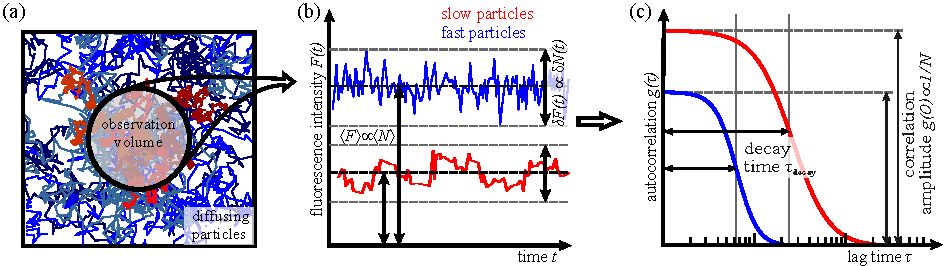
\includegraphics{pic/fcs_principle.pdf}
	\mycaption{Illustration of the principle of FCS.}{(a) Sample with particles moving with different diffusion coefficients (fast: blue, slow: red). The circle indicates the observation volume. (b) Fluorescence intensity, as measured from the sample in (a), showing the fluorescence fluctuations $\delta F(t)$ around the mean intensity $\mean{F}$. (c) Autocorrelation functions $g(\tau)$, calculated from the intensity traces in (b). The decay times $\taudecay$ are defined by $g(\taudecay)=g(0)/2$. }
	\label{fig:fcs_principle}
\end{figure}

FCS was introduced  in 1974 by \citeauthor*{MAGDE1974} in Refs.~\cite{MAGDE1974, MAGDE1974a,MAGDE1978}. As shown in \figref{fig:fcs_principle}, fluorescence is excited and detected in a tiny subvolume (a few $\unit{\mu m^3}$) of the sample containing only few particles $N(t)$ at any time. The measured fluorescence intensity $F(t)$ is proportional to this particle number. Due to the diffusive motion of the particles, $N(t)$ is permanently fluctuating around its mean value $\mean{N}$. This is represented as:
\begin{equation}\label{eq:fcs_particlenumber}
  N(t)=\mean{N}+\delta N(t)\ \ \ \ \ \Rightarrow\ \ \ \ \ F(t)=\mean{F}+\delta F(t)\ \ \ \ \ \text{with}\ \ \smean{\delta N(t)}=\smean{\delta F(t)}=0.
\end{equation}
Here $\delta N(t)$ and $\delta F(t)$ represent the fluctuations of the particle number and the fluorescence intensity. Depending on the speed of motion (diffusion coefficient), the particle number fluctuates ``faster'' or ``slower''. This can be quantified using an autocorrelation analysis. The normalized FCS autocorrelation function is defined as
\begin{equation}\label{eq:fcs_acf}
  g(\tau)=\frac{\mean{\delta F(t)\cdot\delta F(t+\tau)}}{\mean{F}^2}=\frac{\mean{ F(t)\cdot F(t+\tau)}}{\mean{F}^2}-1,\ \ \ \tau>0.
\end{equation}
where the averaging operation $\mean{\cdot}$ is defined as a a time average:
\begin{equation}\label{eq:fcs_avg}
  \mean{F(t)}=\lim\limits_{T\rightarrow\infty}\frac{1}{T}\cdot\int\limits_0^TF(t)\;\ddt.
\end{equation}
The autocorrelation function $g(\tau)$ measures the similarity of the signal $F(t)$ to its time-shifted version $F(t+\tau)$. If the fluctuations are completely random white noise, the correlation function is $g(\tau)\propto\ddelta(\tau)$, which is $0$ for all time lags $\tau>0$. If $F(t)$ contains a non-random component, the correlation will be non-zero over a lag-time range, which is characteristic for the non-random process. In FCS the non-random fluctuations are caused by Brownian motion of fluorescent particles, which implies a typical dwell time of the particles in the observation volume of\footnote{This equation is related to the mean-squared displacement (MSD) of a particle undergoing \itindex{normal diffusion}, which was shown by Albert Einstein to be $\langle r^2\rangle(\tau)=2\cdot d\cdot D\cdot\tau$, where $d$ is the dimensionality of the motion and $D$ is the \itindex{diffusion coefficient}.}:
\begin{equation}\label{eq:fcs_taudecay}
  \tauD\propto\frac{\left(\sqrt[3]{\Vobs}\right)^2}{D}.
\end{equation}
During this time, the presence of a single particle causes a self-similarity in the fluctuations, which manifests itself as a decay of the autocorrelation function from a zero-lag amplitude $g(0)>0$ to $g(\infty)=0$. The half-life time $\taudecay$ of this decay is approximately given by $\tauD$ from \eqref{eq:fcs_taudecay}.

The zero-lag amplitude $g(0)$ of the autocorrelation function \eqref{eq:fcs_acf} yields the average particle number in the observation volume, as
\begin{equation}\label{eq:fcs_acfn}
  g(0)=\frac{\smean{\delta F^2(t)}}{\mean{F}^2}\propto\frac{\smean{\delta N^2(t)}}{\mean{N}^2}=\frac{1}{\mean{N}}.
\end{equation}
In the last step, the Poissonian nature of the randomly fluctuating particle number $N(t)$ was used, which dictates that $\smean{\delta^2 N(t)}\equiv\Var(N(t))=\mean{N}$.



Today FCS is typically implemented using confocal microscopes with a very small observation volume ($\Vobs\approx0.2-0.6\unit{\mu m^3}$), and fluorescence is detected by  single-photon avalanche diodes (SPADs or simply APDs). The acquired fluorescence intensity time-trace $F(t)$ is  correlated using either specialized digital electronics or a software correlator. In a final step, analytical model functions are used to determine the average particle number $\mean{N}$, the diffusion coefficient $D$ (via the decay time $\taudecay$) and other properties of the molecular motion, such as flow speeds, anomalous diffusion exponent, kinetic reaction rates. %This combination is available even on commercial confocal microscopes today and has found widespread application in biological and biophysical research (see e.g. Refs.~\cite{KRICHEVS2002,HAUSTEIN2007,LIU2008a,ELSON2011,TIAN2011,WOELL2013} for reviews of the technique in different field).


\section{Modeling fluorescence in a microscope}
\label{sec:FCSModelingTheOpticalSystem}

%FCS model functions should represent results that are obtained from a real-world microscope exciting and detecting fluorescence from randomly moving particles.  So in a first step this process has to be modeled. The simplification of a microscope used in this chapter, is illustrated in \figref{fig:fcs_microscopeschematic}. 
\begin{figure}[t!]
	\centering
		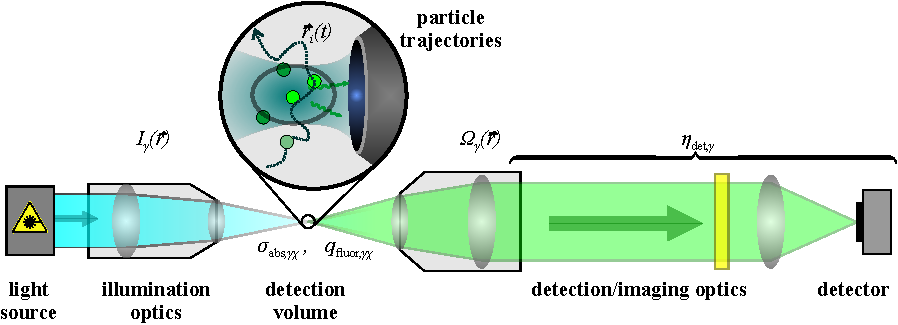
\includegraphics{pic/fcs_microscopeschematic.pdf}
	\mycaption{Schematic of the optics model used for the derivation of FCS theory.}{The illumination optics focuses light into an intensity distribution $I_\gamma(\vr)$. The detection optics is characterized by its detection probability distribution $\Omega_\gamma(\vr)$ and the detection efficiency $\etadetgamma$. The sample is modeled as a set of particles with trajectories $\vr_i(t)$. To each species an absorption cross-section $\sigmaabsgammachi$ and a fluorescence quantum efficiency $\qfluorgammachi$ is assigned. }
  %The microscope is split into its functional components: The light source and illumination optics (illumination profile $I_\gamma(\vr)$), the detection optics (detection probability distribution $\Omega_\gamma(\vr)$) and the detector itself (detection efficiency $\etadetgamma$, summarizing the detector and the detection  optics). The color channel is encoded by the index $\gamma$. The sample itself is modeled as a set of particles $i$ of species $\chi$, following trajectories $\vr_i(t)$. To each species a absorption crosssection $\sigmaabsgammachi$ and a fluorescence quantum efficiency $\qfluorgammachi$ is assigned.}
	\label{fig:fcs_microscopeschematic}
\end{figure}

%In order to 
The theoretical framework of FCS starts from a simplified model of the fluorescence microscope, which is used to acquire the data. \Figref{fig:fcs_microscopeschematic} illustrates this model. It will be explained in detail throughout this section.

The sample of volume $\Vsample$ contains $\Nsamplechi$ particles of species $\chi$ that move randomly. The motion of each particle $i=1...\Nsample(\chi)$ is described by its trajectory $\vr_i(t)$. The trajectories are typically not known exactly, but their statistics, such as the \itindex{mean squared displacement (MSD)}\index{MSD}, is known. Finally, the local particle concentration distribution of species $\chi$ can be written as
\begin{equation}\label{eq:fcstheory_concentration}
  c_\chi(\vr,t)=\frac{1}{\Vsample}\cdot\sum\limits_{i=1}^{\Nsamplechi}\ddelta\bigl[\vr-\vr_i(t)\bigr].
\end{equation}

The particles are illuminated by some kind of illumination optics (e.g. a \itindex{confocal microscope} or a \itindex{selective plane illumination microscope (SPIM)}\index{SPIM}) with an intensity distribution $I_\gamma(\vr)$. The index $\gamma\in\{\txt{g},\txt{r}, ...\}$ denotes the color channel of the microscope, e.g. $\gamma=\txt{g}$ for excitation at $488\unit{nm}$ and detection in the range of $[500...550]\unit{nm}$ to observe eGFP, or $\gamma=\txt{r}$ for excitation at $568\unit{nm}$ and detection at $[600...700]\unit{nm}$ for mRFP. An absorption cross-section $\sigmaabsgammachi$ and a fluorescence quantum yield $\qfluorgammachi$ is assigned to each species. Then the amount of fluorescence emitted by a single fluorophore of species $\chi$ at position $\vr$ into channel $\gamma$ can be written as
  \[ I_\gamma(\vr)\cdot\sigmaabsgammachi\cdot\qfluorgammachi. \]
The detection optics is described by a detection efficiency distribution $\Omega_\gamma(\vr)$ and a detection efficiency $\etadetgamma$. The latter summarizes any signal loss due to optical surfaces or filters in the detection beam path. The distributions $I_\gamma(\vr)$ and $\Omega_\gamma(\vr)$ are not observable independently, so they are usually combined into a single function, called \itindex{molecular detection efficiency (MDE)}\index{MDE}:
\begin{equation}\label{eq:fcstheory_mde}
  \MDE_\gamma(\vr):=I_\gamma(\vr)\cdot\Omega_\gamma(\vr).
\end{equation}
This function is proportional to the rate of fluorescence photons expected from a fluorophore at position~$\vr$. Its actual form for a given microscopy setup can be calculated from the PSFs of the microscope. The geometry of the detectors (e.g. square pixels of a camera) also may need to be taken into account. For confocal setups a 3-dimensional, rotationally symmetric Gaussian function with width $w_\gamma$ and height $z_\gamma$ is a good approximation:
\begin{equation}\label{eq:fcstheory_mde_confocal}
  \MDE_{\txt{confocal,} \gamma}(\vr)=I_0\cdot\exp\left(-2\cdot\frac{x^2+y^2}{w_\gamma^2}-2\cdot\frac{z^2}{z_\gamma^2}\right).
\end{equation}



In Refs.~\cite{WOHLAND2010,SINGHKRIEGER2013,KRIEGERPHD2014} it is argued, that a properly designed and aligned SPIM has a PSF with negligible sidelobe contributions. So the PSF can also be approximated by a Gaussian function. Still the finite size of the quadratic camera pixel has to be taken into account for the final form of the MDE:
\begin{equation}\label{eq:fcstheory_mde_SPIM_int}
  \MDE_{\txt{SPIM,} \gamma}(\vr)=I_0\cdot (h_\txt{pixel}\conv\PSF_{\txt{SPIM,} \gamma})(\vr)=\iint\limits_{-\pixelsize/2\ \ }^{\ \ \pixelsize/2} \PSF_{\txt{SPIM,} \gamma}(\vr-\vr')\;\ddxs\;\ddys,
\end{equation}
where $\pixelsize$ is the width of the pixel in the object plane, $\conv$ denotes convolution and $h_\txt{pixel}(\vr)$ is the characteristic function, describing a camera pixel:
\begin{equation}\label{eq:imaging_CEF}
  h_\txt{pixel}(\vr)=\ddelta(z)\cdot\begin{cases}1 & -\frac{\pixelsize}{2}\leq x\leq\frac{\pixelsize}{2}\ \ \ \wedge\ \ \ -\frac{\pixelsize}{2}\leq y\leq\frac{\pixelsize}{2}\\ 0 & \text{else}\end{cases}.
\end{equation}
The convolution integral in \eqref{eq:fcstheory_mde_SPIM_int} can be solved analytically:
\begin{equation}\label{eq:fcstheory_mde_SPIM}
 \MDE_{\txt{SPIM,} \gamma}(\vr)=I_0\cdot\frac{\left[\erf\left(\frac{\pixelsize-2x}{\sqrt{2}\cdot w_\gamma}\right)+\erf\left(\frac{\pixelsize+2x}{\sqrt{2}\cdot w_\gamma}\right)\right]\cdot\left[\erf\left(\frac{\pixelsize-2y}{\sqrt{2}\cdot w_\gamma}\right)+\erf\left(\frac{\pixelsize+2y}{\sqrt{2}\cdot w_\gamma}\right)\right]}{\left[2\cdot\erf\left(\frac{\pixelsize}{\sqrt{2}\cdot w_\gamma}\right)\right]^2}\cdot\exp\left(-2\cdot\frac{z^2}{z_\gamma^2}\right)
\end{equation}
As shown in \figref{fig:pixel_psf_cut}, this MDE deviates significantly from a Gaussian function, if $\pixelsize$ is significantly larger than the size $w_\gamma$ of the PSF. 

%Throughout the rest of this chapter, results are typically given in two form. For a Gaussian MDE in \eqref{eq:fcstheory_mde_confocal} and for the SPIM MDE in \eqref{eq:fcstheory_mde_SPIM}.


\begin{figure}[t!]
	\centering
    \begin{gnuplot}[terminal=\defaultgnuplotterminal,terminaloptions=\defaultgnuplotterminalopts{14cm}{5cm},preamble=\defaultgnuplotpreamble]
      set xlabel 'positions $x\unitbs{\mu m}$'
      set ylabel '$\MDE_{\txt{SPIM,} \gamma}(x)$ [A.U.]'
      set samples 500
      #set palette rgb 23,28,3;
      unset colorbox
      set key outside rmargin
      MDE(x,w,a)=(erf((a-2.0*x)/(sqrt(2.0)*w))+erf((a+2.0*x)/(sqrt(2.0)*w)))/(2.0*erf(a/(sqrt(2)*w)))
      G(x,w)=exp(-2.0*x*x/w/w)
      plot [-3.5:3.5][0:1.1] MDE(x,0.5,0.5) title 'SPIM MDE: $a=500\unit{nm}$' with lines lc palette frac 0.0, \
                  MDE(x,0.5,1) title 'SPIM MDE: $a=1000\unit{nm}$' with lines lc palette frac 0.3, \
                  MDE(x,0.5,2) title 'SPIM MDE: $a=2000\unit{nm}$' with lines lc palette frac 0.6, \
                  MDE(x,0.5,4) title 'SPIM MDE: $a=4000\unit{nm}$' with lines lc palette frac 1, \
                  G(x,0.5) title 'Gaussian' with lines lc rgbcolor "red"
    \end{gnuplot}

	\mycaption{Plots of cuts through the MDE of a SPIM in \eqref{eq:fcstheory_mde_SPIM} along one coordinate axis.}{ For all plots, the PSF width was $w_\gamma=500\unit{nm}$.}
	\label{fig:pixel_psf_cut}
\end{figure}

Finally, the results of this section can be combined into the fluorescence time trace expected from a fluorophore concentration $c_\chi(\vr,t)$ (see \eqref{eq:fcstheory_concentration}):
\begin{equation}\label{eq:fcstheory_fluorescence_raw}
  F_\gamma(t)=\fullvolint\MDE_\gamma(\vr)\cdot\sum\limits_{\chi\in\bbS}\etadetgamma\cdot\sigmaabsgammachi\cdot\qfluorgammachi\cdot c_\chi(\vr,t)\;\ddV.%\etagammachi
\end{equation}
The factors $\etadetgamma$, $\sigmaabsgammachi$ and $\qfluorgammachi$ are not distinguishable in a FCS experiment, so they are summarized into a single detection efficiency $\etagammachi$ of a fluorophore of species $\chi\in\bbS$ in channel $\gamma$:
\begin{equation}\label{eq:fcstheory_etagammachi}
  \etagammachi\equiv\etadetgamma\cdot\sigmaabsgammachi\cdot\qfluorgammachi
\end{equation}
Then \eqref{eq:fcstheory_fluorescence_raw} can be simplified to
\begin{equation}\label{eq:fcstheory_fluorescence}
  F_\gamma(t)=\fullvolint\MDE_\gamma(\vr)\cdot\sum\limits_{\chi\in\bbS}\etagammachi\cdot c_\chi(\vr,t)\;\ddV.
\end{equation}
As shown in \eqref{eq:fcs_acf}, the autocorrelation function is written in terms of signal fluctuations $\delta F_\gamma(t)$ around a mean intensity $\smean{F_\gamma}$. These can be expressed in a form analogous to \eqref{eq:fcstheory_fluorescence}, if the concentration dynamics $c_\chi(\vr,t)$ is also split into a fluctuation part and  an average concentration:%,  constant over the size of the MDE and the time of the measurement:
\begin{equation}\label{eq:fcstheory_concfluc}
  c_\chi(\vr,t)=\smean{c_\chi}+\delta c_\chi(\vr,t).
\end{equation}
Due to the linearity of \eqref{eq:fcstheory_fluorescence}, this finally yields:
\begin{equation}\label{eq:fcstheory_fluorescencefluc}
  \delta F_\gamma(t)=\fullvolint\MDE_\gamma(\vr)\cdot\sum\limits_{\chi\in\bbS}\etagammachi\cdot \delta c_\chi(\vr,t)\;\ddV.
\end{equation}
%The mean fluorescence signal can be simplified to:
%\begin{equation}\label{eq:fcstheory_meanfluorescence}
%  \mean{F_\gamma}= \sum\limits_{\chi\in\bbS}\etagammachi\fullvolint\MDE_\gamma(\vr)\cdot \mean{c_\chi(\vr)}\;\ddV,= \sum\limits_{\chi\in\bbS}\etagammachi \mean{N_\chi},
%\end{equation}
%where $\smean{N_\chi}$ is the mean number of particles of species $\chi$ in the focal volume, defined by the MDE. In this form the meaning of $\etagammachi$ is simply molecular brightness, i.e. the average amount of fluorescence emitted a single particle of species $\chi$ int the observation volume. 


%Also the MDE is required to be normalized:
%\begin{equation}\label{eq:fcstheory_mde_normalized}
%  \fullvolint\MDE_{\gamma}(\vr)\;\ddV\overset{!}{=}1.
%\end{equation}
%This normalization condition will be used throughout the rest of this thesis, as it simplifies some derivations. As all correlation functions are normalized to the average intensity, the global normalization factor imposed by \eqref{eq:fcstheory_mde_normalized} will not influence the final results. Care has to be taken in order to interpret all other properties are accordingly.



\section{Theory of fluorescence correlation spectroscopy}
\label{sec:ConfocalFluorescenceCorrelationSpectroscopy}
\subsection{The FCS autocorrelation function}
\label{sec:TheFCSAutocorrelationFunctionTheory}


\noindent For a color channel $\gamma$, the FCS autocorrelation function is defined as
\begin{equation*}
  g_\gamma(\tau)=\frac{\mean{\delta F_\gamma(t)\cdot\delta F_\gamma(t+\tau)}}{\mean{F_\gamma}^2}. \tag{\ref{eq:fcs_acf}}
\end{equation*}
Using the results in \eqsref{eq:fcstheory_fluorescence}{eq:fcstheory_fluorescencefluc} this can be rewritten as:
\begin{equation}\label{eq:fcs_acffull}
  g_\gamma(\tau)=\frac{\sum\limits_{\chi\in\bbS}\etagammachi^2 \fullvolint\fullvolint\MDE_\gamma(\vr)\cdot\MDE_\gamma(\vr')\cdot\mean{\delta c_\chi(\vr,t)\cdot\delta c_\chi(\vr',t+\tau)}\;\ddV\ddV' }{\left(\sum\limits_{\chi\in\bbS}\etagammachi \cdot\fullvolint\MDE_\gamma(\vr)\cdot \mean{c_\chi(\vr,t)}\;\ddV\right)^2}.
\end{equation}
Here, the linearity of the integration and averaging $\smean{\cdot}$ was used. Furthermore, it was assumed that the concentration fluctuations from two different molecular species $\chi$ and $\chi'$ are statistically independent, i.e. $\smean{\delta c_\chi(\vr,t)\cdot\delta c_{\chi'}(\vr,t)}=0$.

\subsection{Zero-lag correlation and particle numbers}
\label{sec:ZeroLagCorrelationAndEffectiveVolume}
%As a first result, an extended form of the statement in \eqref{eq:fcs_acfn} on the zero-lag amplitude of the autocorrelation function $g(0)\propto 1/\mean{N}$ can be made, using again 
The Poissonian nature of the particle number (or concentration) in the focus dictates for $\tau=0$:
\begin{equation}\label{eq:fcs_zerolagconcentrationcorrelation}
  \mean{\delta c_\chi(\vr,t)\cdot\delta c_\chi(\vr',t)}\equiv\mean{\delta c_\chi^2(\vr,t)}\cdot\ddelta(\vr-\vr')=\mean{c(\vr,t)}\cdot\ddelta(\vr-\vr'),
\end{equation}
where the factor $\ddelta(\vr-\vr')$ signifies, that single particles are non-interacting and therefore, also statistically independent. Therefore they are only correlated to themselves and not to other particles nearby. 
Using \eqref{eq:fcs_zerolagconcentrationcorrelation} and further assuming that the concentration does not change significantly over the observation volume (described by the MDE), i.e. $\smean{c_\chi(\vr)}\equiv\smean{c_\chi}$, the zero-lag autocorrelation amplitude becomes: %\eqref{eq:fcs_acffull} can be further simplified for $\tau=0$:
\begin{multline}\label{eq:fcs_acffull_zerolag}
  g_\gamma(0)=\frac{\sum\limits_{\chi\in\bbS}\etagammachi^2\cdot\smean{c_\chi}\cdot \fullvolint\MDE_\gamma^2(\vr)\;\ddV }{\left(\sum\limits_{\chi\in\bbS}\etagammachi \cdot\smean{c_\chi}\cdot\fullvolint\MDE_\gamma(\vr)\;\ddV\right)^2}=\\
  =\frac{\sum\limits_{\chi\in\bbS}\etagammachi^2\cdot\smean{c_\chi} }{\left(\sum\limits_{\chi\in\bbS}\etagammachi \cdot\smean{c_\chi}\right)^2}\cdot\frac{\fullvolint\MDE_\gamma^2(\vr)\;\ddV}{\left(\fullvolint\MDE_\gamma(\vr)\;\ddV\right)^2}\underset{\bbS=\{\chi\}}{=} \frac{1 }{\smean{c_\chi}}\cdot\frac{\fullvolint\MDE_\gamma^2(\vr)\;\ddV}{\left(\fullvolint\MDE_\gamma(\vr)\;\ddV\right)^2}.
\end{multline}
In the last step, a single species $\chi$ was assumed. %If the last fraction in this result is interpreted as an inverse volume, i.e.
Introducing the effective volume %$\Veffm{\gamma}$
\begin{equation}\label{eq:fcs_Veff}
  \Veffm{\gamma}:=\frac{\left(\fullvolint\MDE_\gamma(\vr)\ddV\right)^2}{\fullvolint\MDE_\gamma^2(\vr)\ddV}
\end{equation}
 of the MDE, the zero-lag amplitude of the autocorrelation function can be written in terms of a particle number $\smean{N_\chi}=\smean{c_\chi}\cdot\Veffm{\gamma}$ within this volume:
\begin{equation}\label{eq:fcs_acf_zerolag}
  g_\gamma(0)=\frac{\sum\limits_{\chi\in\bbS}\etagammachi^2\cdot\smean{c_\chi}\cdot\Veffm{\gamma} }{\left(\sum\limits_{\chi\in\bbS}\etagammachi \cdot\smean{c_\chi}\cdot\Veffm{\gamma}\right)^2} =\frac{\sum\limits_{\chi\in\bbS}\etagammachi^2\cdot\mean{N_\chi} }{\left(\sum\limits_{\chi\in\bbS}\etagammachi \cdot\mean{N_\chi}\right)^2}\underset{\bbS=\{\chi\}}{=}\frac{1}{\mean{N_\chi}}.
\end{equation}

For confocal and light sheet microscopes, the MDEs were defined in section \ref{sec:FCSModelingTheOpticalSystem}. The integrals in the effective volume in \eqref{eq:fcs_Veff} can be calculated analytically for these specific MDEs:
\begin{align}
   \text{confocal:} \ \ \ \ \ \ \Veffm{\gamma}&=\pi^{3/2}\cdot w_\gamma^2\cdot z_\gamma,\label{eq:fcs_Veff_confocal}\\
   \text{SPIM:} \ \ \ \ \ \ \Veffm{\gamma}&= \frac{\sqrt{\pi}\cdot \pixelsize^{2}\cdot z_\gamma}{\left[\erf\left(\frac{\pixelsize}{w_\gamma}\right)+\frac{w_\gamma}{\sqrt\pi\cdot \pixelsize}\left(\ee^{-\pixelsize^2/w_{\gamma}^2}-1\right)\right]^2}.\label{eq:fcs_Veff_SPIM}
\end{align}


\subsection{The concentration correlation factor}
\label{sec:TheConcentrationCorrelationFactor}
\noindent In the autocorrelation function \eqref{eq:fcs_acffull} the particle dynamics is fully described by the concentration correlation factor 
\begin{equation}\label{eq:fcs_corrfactordef}
    \mean{\delta c_\chi(\vr,t)\cdot\delta c_\chi(\vr',t+\tau)}=:\phi_\chi(\vr,\vr',\tau)\equiv \phi_\chi(\vr-\vr',\tau).
\end{equation}
It quantifies the amount of correlation at a time-lag $\tau$ between the concentration fluctuations at two positions $\vr$ and $\vr'$. The last equivalence in \eqref{eq:fcs_corrfactordef} states that $\phi_\chi(\cdot,\cdot)$ only depends on the difference in positions, i.e. the whole system is shift-invariant in space. If the system of interest is furthermore isotropic, the self correlation function only depends on the length $\snorm{\vr-\vr'}$, i.e. \mbox{$\phi_\chi(\vr,\vr',\tau)\equiv \phi_\chi(\snorm{\vr-\vr'},\tau)$}. Note that generally these assumptions are not necessarily true, but on the small scales of FCS measurements they usually are assumed to apply.

%As stated in \eqref{eq:fcs_zerolagconcentrationcorrelation}, initially ($\tau=0$) correlation has not spread over space yet and thus the correlation factor is proportional to $\ddelta(\vr-\vr')$. For an arbitrary time lag $\tau$, it has to be calculated from the equations of motion of the modeled system, e.g. the diffusion differential equation \deqref{eq:intro_diffusion_dgl}.

The concentration correlation factor is (up to prefactors) equivalent to the van-Hove self correlation function of the particles \cite{HANSEN2013,HOPKIN2010,HOFLIN2013}, which is given in terms of single-particle trajectories $i=1,2,...,N$ as \cite{HOPKIN2010}:
\begin{align}\label{eq:fcs_vanhove_trajectory}
    P_\chi(\vr,\vr',\tau)&=\frac{1}{N}\cdot\mean{\sum\limits_{i=1}^N\ddelta(\vr'-\vr+\vr_i(0)-\vr-(\vr_i(\tau)-\vr)}.
\end{align}
Here, $P_\chi(\cdot,\cdot,\cdot)$ can be interpreted as the probability to find a particle at position $\vr'$ at time $\tau$, if it was initially at position $\vr$. Specific forms of $P_\chi(\cdot,\cdot)$ can be calculated as the Green's function or propagator of the \itindex{photon detection efficiency (PDE)}\index{PDE}, which governs the dynamics of $c_\chi(\vr,t)$. A simple example for the PDE is the \itindex{diffusion equation} in 
  \begin{equation}\label{eq:intro_diffusion_dgl}  
    \fracpd{c(\vr, t)}{t}= D\cdot \vnabla^2c(\vr, t),
  \end{equation}
where $D$ is the \itindex{diffusion coefficient}.
%In that framework, $\phi_\chi(\cdot,\cdot)$ equals the Green's function, or propagator $P_\chi(\vr,\vr',\tau)$ of the PDE. 
The Green's function is defined as the solution of the PDE for the initial condition $c_\chi(\vr,0)=\ddelta(\vr)$ \cite{BOAS1983}. It can be used to calculate the solution $c_\chi(\vr,\tau)$ of the PDE for an arbitrary initial condition $c_\chi(\vr,0)$ at any time $\tau>0$:
\begin{equation}\label{eq:intro_diffusion_dgl_solution_greens}  
  c_\chi(\vr,\tau)=c_\chi(\vr,0)\conv P_\chi(\vr,\tau)=\idotsint c_\chi(\vr',0)\cdot P_\chi(\vr,\vr',\tau)\;\dd^\ddim r'.
\end{equation}
Here $\conv$ denotes a convolution and $\ddim$ is the dimension of the space, in which the motion takes place. Finally, the concentration correlation factor is given by
\begin{equation}\label{eq:fcs_diffusion_vanHove_and_Propagator}  
  \phi_\chi(\vr,\vr',\tau)=\mean{\delta c_\chi(\vr,t)\cdot\delta c_\chi(\vr',t+\tau)}=\smean{c_\chi}\cdot P_\chi(\vr,\vr',\tau).
\end{equation}


\noindent With these definitions, \eqref{eq:fcs_acffull} can be slightly rewritten:
\begin{multline}\label{eq:fcs_acffull_phifactor}
  g_\gamma(\tau)=\frac{\sum\limits_{\chi\in\bbS}\etagammachi^2 \smean{c_\chi}\fullvolint\fullvolint\MDE_\gamma(\vr)\cdot\MDE_\gamma(\vr')\cdot\phi_\chi(\vr,\vr',\tau)\;\ddV\ddV' }{\left(\sum\limits_{\chi\in\bbS}\etagammachi \smean{c_\chi}\right)^2\cdot\left(\fullvolint\MDE_\gamma(\vr)\;\ddV\right)^2}=\\
  =\frac{\sum\limits_{\chi\in\bbS}\etagammachi^2 G_{\gamma}^{\chi}(\tau) }{\left(\sum\limits_{\chi\in\bbS}\etagammachi \smean{c_\chi}\right)^2}.
\end{multline}
In this form a non-normalized correlation function
\begin{multline}\label{eq:fcs_nnormacf}
  G_{\gamma}^{\chi}(\tau):=\frac{\mean{\delta F_\gamma^{\chi}(t)\cdot\delta F_\gamma^{\chi}(t+\tau)}}{\etagammachi^2\cdot\left(\fullvolint\MDE_\gamma(\vr)\;\ddV\right)^2}=\\
  =\smean{c_\chi}\cdot\frac{\fullvolint\fullvolint\MDE_\gamma(\vr)\cdot\MDE_\gamma(\vr')\cdot\phi_\chi(\vr,\vr',\tau)\;\ddV\ddV'}{\left(\fullvolint\MDE_\gamma(\vr)\;\ddV\right)^2}
\end{multline}
of the fluctuations $\delta F_\gamma^{\chi}(t)$ caused by a single species $\chi$ in a channel $\gamma$ is introduced.


%Now the problem of calculating the FCS autocorrelation function for a given situation is reduced to finding the van-Hove self correlation function. In many cases, the dynamics is governed by a linear (partial) differential equation. Then its solution $\delta c_\chi(\vr,t+\tau)$ is given by the Green's function or propagator $P(\vr,\vr',\tau)$ of the equations of motion and an initial condition $\delta c_\chi(\vr,t)$ \cite{BOAS1983}:
  %\[ \delta c_\chi(\vr,t+\tau)=\delta c_\chi(\vr,t)\conv P(\vr,\vr', \tau) \]
%In that case the van Hove self correlation function is generally given by:
%\begin{equation}\label{eq:fcs_diffusion_vanHove_and_Propagator}  
  %\phi_\chi(\vr,\vr',\tau)=\mean{\delta c_\chi(\vr,t)\cdot\delta c_\chi(\vr',t+\tau)}=\smean{c_\chi}\cdot P_\chi(\vr,\vr',\tau).
%\end{equation}
%This result can be derived, using that in reciprocal Fourier space (see appendix~\ref{sec:FourierTransform}) the convolution translates to a multiplication:
%\begin{align*}
  %\phi_\chi(\vr,\vr',\tau)&=\mean{\delta c_\chi(\vr,t)\cdot\delta c_\chi(\vr',t+\tau)}=\mean{\delta c_\chi(\vr,t)\cdot\left[\delta c_\chi(\vr',t)\conv P(\vr,\vr',\tau)\right]}=\\
  %&=\mean{\FTia[\vk']{\delta c_\chi(\vr,t)\cdot\delta \tilde c_\chi(\vk',t+\tau)}}=\FTia[\vk']{\mean{\delta c_\chi(\vr,t)\cdot\delta \tilde c_\chi(\vk',t)}\cdot\tilde P_\chi(\vr,\vk',\tau)}=\\
  %&=\mean{\delta c_\chi(\vr,t)\cdot\delta c_\chi(\vr',t)}\conv P_\chi(\vr,\vr',\tau)
%\end{align*}
%Here $\tilde{f}(\vk)$ is the Fourier transform of a function $f(\vr)$ and $f(\vr)=\FTia[\vk]{\tilde f(\vk)}$ denotes inverse Fourier transform. Linearity of Fourier transform and averaging allows one to exchange the two operations. Note in the second line, that the factor $\tilde P_\chi(\vr,\vk',\tau)$ does not depend on the absolute time $t$, so it can be written outside the time-average $\mean{\cdot}$. Finally using the $\ddelta$-function in \eqref{eq:fcs_zerolagconcentrationcorrelation}, the last line of equations can be rewritten in a simple form:
%\begin{equation*}
  %\phi_\chi(\vr,\vr',\tau)=\mean{\delta c_\chi(\vr,t)\cdot\delta c_\chi(\vr',t+\tau)}=\smean{c_\chi}\cdot P_\chi(\vr,\vr',\tau).\tag{\ref{eq:fcs_diffusion_vanHove_and_Propagator}  }
%\end{equation*}
%This result was derived, starting from the diffusion equation, but it is generally true, as long as $\delta c_\chi(\vr,t+\tau)$ can be written as a convolution of $\delta c_\chi(\vr,t)$ with a propagator $P(\vr,\vr',\tau)$, because the actual form of the diffusion equation was never used.

The next subsections will give the exact mathematical form of $\phi_\chi(\vr,\vr',\tau)$ and the FCS autocorrelation functions $G_{\gamma}^{\chi}(\tau)$ and $g(\tau)$ for different situations frequently encountered in FCS measurements.



\subsection{Normal diffusion}\index{normal diffusion}\index{diffusion}
\label{sec:NormalDiffusionFCS}
The most common dynamics in FCS is normal diffusion. Here, the particle concentration dynamics $c_\chi(\vr,t)=\smean{c_\chi}+\delta c_\chi(\vr,t)$ is governed by the \itindex{diffusion equation} \eqref{eq:intro_diffusion_dgl}:
\begin{equation}\label{eq:fcs_diffusion_dgl_fluctuations}  
  \fracpd{\left(\smean{c_\chi}+\delta c_\chi(\vr, t)\right)}{t}=D_\chi\cdot \vnabla^2\left(\smean{c_\chi}+\delta c_\chi(\vr, t)\right)\ \ \ \ \ \Rightarrow\ \ \ \ \ \ \fracpd{\delta c_\chi(\vr, t)}{t}=D_\chi\cdot \vnabla^2\delta c_\chi(\vr, t).
\end{equation}
The Green's function of the this PDE \eqref{eq:fcs_diffusion_dgl_fluctuations} is
\begin{equation}\label{eq:fcs_ndiff_propagator}
  P_\chi(\vr,\vr',\tau)=\frac{1}{\Bigl(4\pi D_\chi\tau\Bigr)^{3/2}}\cdot\exp\left(-\frac{(\vr'-\vr)^2}{4D_\chi\tau}\right).
\end{equation}
Note that the \itindex{diffusion equation} \eqref{eq:intro_diffusion_dgl} (and likewise \eqref{eq:fcs_diffusion_dgl_fluctuations}) can be interpreted statistically and then also a single-particle \itindex{mean squared displacement (MSD)} can be calculated. For normal diffusion in $d$ dimensions, Albert Einstein derived:
\begin{equation}\label{eq:msd_normal_diffusion}
  \MSD(\tau)\equiv\langle r^2\rangle(\tau)=2d\cdot D\cdot\tau.
\end{equation}


%Using this, the FCS autocorrelation functions can be calculated analytically from \eqref{eq:fcs_nnormacf}, provided that the MDE is sufficiently. Especially in the case of the MDEs given in \eqref{eq:fcs_Veff_confocal} and \eqref{eq:fcs_Veff_SPIM}, the volume integrals separate into three independent coordinate directions, so the non-normalized correlation function reads:
With this result and the MDEs in \eqsref{eq:fcs_Veff_confocal}{eq:fcs_Veff_SPIM}, the FCS autocorrelation function for normal diffusion can be calculated. The MDEs as well as \eqref{eq:fcs_ndiff_propagator} can be separated into three factors that depend solely on a single direction $x$, $y$ or $z$. Therefore, also the autocorrelation function separates into three directional components:
\begin{equation}\label{eq:fcs_ndiff_cc_separated}
  G_{\gamma}^{\chi}(\tau)=\smean{c_\chi}\cdot G_{\gamma,x}^{\chi}(\tau)\cdot G_{\gamma,y}^{\chi}(\tau)\cdot G_{\gamma,z}^{\chi}(\tau).
\end{equation}
Each directional factor is defined by
\begin{equation}\label{eq:fcs_ndiff_cc_separated_dirfactor}
   G_{\gamma,x}^{\chi}(\tau)=\frac{\int\limits_{-\infty}^\infty\int\limits_{-\infty}^\infty\MDE_{\gamma,x}(\xi)\cdot\MDE_{\gamma,x}(\xi')\cdot\phi_{\chi,x}(\xi,\xi',\tau)\dd\xi\dd\xi'}{\left(\int\limits_{-\infty}^\infty\MDE_x(\xi)\dd\xi\right)^2}.
\end{equation}
Here the directional components of $\MDE_\gamma(\vr)$ and of  $\phi_\chi(\vr,\vr',\tau)$ are denoted by an additional index $x$.


For a 3-dimensional Gaussian MDE (\eqrefn{eq:fcstheory_mde_confocal}), the directional factor in \eqref{eq:fcs_ndiff_cc_separated_dirfactor} is given for the $x$ and $y$ direction by%for directions $x$ or $y$ with the associated MDE-width $w_\gamma$ (or $z$ with width $z_\gamma$ by replacement) is
\begin{equation}\label{eq:fcs_ndiff_cc_confocal_separated_factor}
  G_{\gamma,x}^{\chi}(\tau)=\frac{1}{\sqrt{\pi}\cdot w_\gamma}\cdot\left(1+\frac{4D_\chi\tau}{w_\gamma^2}\right)^{-1/2}.
\end{equation}
The factor for the $z$ direction is of the same form, but with $w_\gamma$ replaced by  $z_\gamma$.
From this the non-normalized correlation function is easily calculated:
\begin{equation}\label{eq:fcs_ndiff_cc_confocal}
  G_{\gamma}^{\chi}(\tau)=\frac{\smean{c_\chi}}{\pi^{3/2}w_\gamma^2 z_\gamma}\cdot\left(1+\frac{4D_\chi\tau}{w_\gamma^2}\right)^{-1}\cdot\left(1+\frac{4D_\chi\tau}{z_\gamma^2}\right)^{-1/2}.
\end{equation}
The final FCS normalized correlation function is then given by:
\begin{equation}\label{eq:fcs_ndiff_confocal}
  g_{\gamma}(\tau)=\frac{1}{\smean{c_\chi}\cdot\pi^{3/2}w_\gamma^2 z_\gamma}\cdot\left(1+\frac{4D_\chi\tau}{w_\gamma^2}\right)^{-1}\cdot\left(1+\frac{4D_\chi\tau}{z_\gamma^2}\right)^{-1/2},
\end{equation}
which can be reformulated to
\begin{equation}\label{eq:fcs_ndiff_confocal_NTauD}
  g_{\gamma}(\tau)=\frac{1}{\smean{N_\chi}}\cdot\left(1+\frac{\tau}{\tauDm{\chi}}\right)^{-1}\cdot\left(1+\frac{\tau}{(z_\gamma/w_\gamma)^2\cdot\tauDm{\chi}}\right)^{-1/2}.
\end{equation}
Here $\smean{N_\chi}$ is the average number of particles in a focal volume as given by \eqref{eq:fcs_Veff_confocal} and $\tauDm{\chi}$ is the diffusion correlation time with
\begin{equation}\label{eq:fcs_ndiff_confocal_tauD}
  \tauDm{\chi}=\frac{w_\gamma^2}{4D_\chi}.
\end{equation}
This $\tauDm{\chi}$ is the average dwell time of particles in the observation volume and also the half decay time of $g_\gamma(\tau)$. \Figref{fig:fcs_confocal_acf_3ddiff_confocal} illustrates the function $g_\gamma(\tau)$ for a single species $\chi$ for different the diffusion coefficients and the particle numbers. The red lines in \figrefs{fig:fcs_confocal_acf_3ddiff_confocal}{a} indicate $\tauDm{\chi}$ for the different cases. They demonstrate that $g_\gamma(\tauDm{\chi}) =g_\gamma(0)/2$. \Figrefs{fig:fcs_confocal_acf_3ddiff_confocal}{b} illustrates the general dependence $g_\gamma(0)=1/\smean{N_\chi}$ of the zero-lag amplitude on the average particle number $\smean{N_\chi}$ in the focal volume.


\begin{figure}[t!]
	\centering
	\begin{minipage}{164mm}\small
		\begin{minipage}{82mm}(a)\\[-3mm]
			\begin{gnuplot}[terminal=\defaultgnuplotterminal,terminaloptions=\defaultgnuplotterminalopts{8cm}{6cm},preamble=\defaultgnuplotpreamble]
			  set format x '\footnotesize $10^{%T}$';
        w=0.25
        gamma=6
        N=10
        tD(D)=w*w/4.0/D
			  g(tau, tauD, N, gamma)=1.0/(1.0+tau/tauD)/sqrt(1.0+tau/tauD/gamma/gamma)/N
			  set logscale x
			  set xlabel 'lag time $\tau\unitb{s}$'
			  set ylabel 'correlation amplitude $g_\gamma(\tau)$'
        #set palette rgb 23,28,3;
        unset colorbox
        set key inside right top vertical  opaque  maxrows 3
        set arrow from 1e-6,g(1,1,N,gamma) to tD(1),g(1,1,N,gamma) nohead fc rgbcolor "light-red"
        set arrow from tD(1),g(1,1,N,gamma) to tD(1),0 nohead fc rgbcolor "light-red"
        set arrow from tD(10),g(1,1,N,gamma) to tD(10),0 nohead fc rgbcolor "light-red"
        set arrow from tD(100),g(1,1,N,gamma) to tD(100),0 nohead fc rgbcolor "light-red"

			  plot [1e-6:10][0:0.105] g(x, tD(100),N,gamma) title '\footnotesize $D_\chi=100\unit{\mu m^2/s}$' with lines lc palette frac 0,  \
                      g(x, tD(10),N,gamma) title '\footnotesize $D_\chi=10\unit{\mu m^2/s}$' with lines lc palette frac 0.5,  \
                      g(x, tD(1),N,gamma) title '\footnotesize $D_\chi=1\unit{\mu m^2/s}$' with lines lc palette frac 1 
			\end{gnuplot}
	  \end{minipage}
		\begin{minipage}{82mm}(b)\\[-3mm]
			\begin{gnuplot}[terminal=\defaultgnuplotterminal,terminaloptions=\defaultgnuplotterminalopts{8cm}{6cm},preamble=\defaultgnuplotpreamble]
			  set format x '\footnotesize $10^{%T}$'; 
        w=0.25
        gamma=6
        D=10
        tD(D)=w*w/4.0/D
			  g(tau, tauD, N, gamma)=1.0/(1.0+tau/tauD)/sqrt(1.0+tau/tauD/gamma/gamma)/N
			  set logscale x
			  set xlabel 'lag time $\tau$ [s]'
			  set ylabel 'correlation amplitude $g_\gamma(\tau)$'
        set key inside right top vertical  opaque width +1 maxrows 3
        #set palette rgb 23,28,3;
        unset colorbox
			  plot [1e-6:10][0:0.21] g(x, tD(D),5,gamma) title '\footnotesize $\langle{N_\chi}\rangle=5$' with lines lc palette frac 0,  \
                      g(x, tD(D),10,gamma) title '\footnotesize $\langle{N_\chi}\rangle=10$' with lines lc palette frac 0.5,  \
                      g(x, tD(D),15,gamma) title '\footnotesize $\langle{N_\chi}\rangle=15$' with lines lc palette frac 1
			\end{gnuplot}
	  \end{minipage}
  \end{minipage}
	\mycaption{Plots of the autocorrelation function for a confocal microscope and 3-dimensional normal diffusion, as defined in \eqref{eq:fcs_ndiff_confocal}.}{In (a) the diffusion coefficient is varied, whereas in (b) the average particle number changes. In (a) the red lines indicate the diffusion correlation time $\tauDm{\chi}$ as defined by \eqref{eq:fcs_ndiff_confocal_tauD} for each of the curves. Fixed parameters: $\smean{N_\chi}=10$, $D_\chi=100\unit{\mu m^2/s}$; MDE parameters: $w_\gamma=250\unit{nm}$, $\kappa_\gamma=6$.}
	\label{fig:fcs_confocal_acf_3ddiff_confocal}
\end{figure}


\paragraph{Lower-dimensional diffusion:} Using the separation of the confocal FCS autocorrelation function into directional components, also lower-dimensional diffusion models are easy to set up. 
In \eqref{eq:fcs_ndiff_cc_separated_dirfactor} one can easily omit the dimensions, along which no motion takes place. 
The concentrations $\smean{c_\chi}$ then have to be reinterpreted as an areal density, or a line density, depending on the diffusion model.



\begin{figure}[t!]
	\centering
  \begin{minipage}{164mm}\small
		\begin{minipage}{82mm}(a)\\[-3mm]
			\begin{gnuplot}[terminal=\defaultgnuplotterminal,terminaloptions=\defaultgnuplotterminalopts{8cm}{6cm},preamble=\defaultgnuplotpreamble]
			  set format x '\footnotesize $10^{%T}$';
        N1=5
        N2=5
        w=0.5
        z=1.2
        a=0.4
        c=10
        D2=1
        D11=100
        D12=10
        D13=2
				sqr(x)=x*x
        gg(tau,D,N)=N/(1.0+4.0*D*tau/w/w)/sqrt(1.0+4.0*D*tau/z/z)
        g(tau, D1, D2, N1, N2)=(gg(tau,D1,N1)+gg(tau,D2,N2))/sqr(N1+N2)
        
        fit g(x,Df1,Df1,N1+N2,0) './data/tau.dat' using ($1):(g($1, D11, D2, N1, N2)) via Df1
        fit g(x,Df2,Df2,N1+N2,0) './data/tau.dat' using 1:(g($1, D12, D2, N1, N2)) via Df2
        fit g(x,Df3,Df3,N1+N2,0) './data/tau.dat' using 1:(g($1, D13, D2, N1, N2)) via Df3
        set logscale x
        set xlabel 'lag time $\tau\unitb{s}$'
        set ylabel 'correlation amplitude $g_\gamma(\tau)$'
        #set palette rgb 23,28,3;
        unset colorbox
        set key inside left bottom vertical  opaque  maxrows 4

        plot [1e-5:10][0:0.105] g(x, D2,   D2, N1, N2) title '\footnotesize 1 component' with lines lt 1 lc rgbcolor "black" lw 1,  \
                                g(x, D11,  D2, N1, N2) title '\footnotesize $D_1=100\unit{\mu m^2/s}$' with lines lc palette frac 0,  \
                                g(x, Df1,  Df1, N1+N2, 0) notitle with lines lt 10 lc palette frac 0 lw 2,  \
                                g(x, D12,  D2, N1, N2) title '\footnotesize $D_1=10\unit{\mu m^2/s}$' with lines lc palette frac 0.3,  \
                                g(x, Df2,  Df2, N1+N2, 0) notitle with lines lt 10 lc palette frac 0.3 lw 2,  \
                                g(x, D13,  D2, N1, N2) title '\footnotesize $D_1=2\unit{\mu m^2/s}$' with lines lc palette frac 0.6 ,  \
                                g(x, Df3,  Df3, N1+N2, 0) notitle with lines lt 10 lc palette frac 0.6 lw 2
                                
			\end{gnuplot}
	  \end{minipage}
		\begin{minipage}{82mm}(b)\\[-3mm]
			\begin{gnuplot}[terminal=\defaultgnuplotterminal,terminaloptions=\defaultgnuplotterminalopts{8cm}{6cm},preamble=\defaultgnuplotpreamble]
			  set format x '\footnotesize $10^{%T}$';
        N=10
        N0=0
        N1=N*0.2
        N2=N*0.4
        N3=N*0.6
        N4=N*0.8
        N5=N
        w=0.5
        z=1.2
        a=0.4
        c=10
        D2=1
        D1=100
        Veff=sqrt(pi)*a*a*z/(erf(a/w)+w/sqrt(pi)/a*(exp(-a*a/w/w)-1.0))**2
        Aeff=a*a/(erf(a/w)+w/sqrt(pi)/a*(exp(-a*a/w/w)-1.0))**2
        tD(D)=Aeff/4.0/D
        sqr(x)=x*x
        gg(tau,D,N)=N/Veff/(sqrt(pi)*a*a*z)*sqr(erf(a/sqrt(4*D*tau+w*w))+sqrt(4*D*tau+w*w)/a/sqrt(pi)*(exp(-a*a/(4*D*tau+w*w))-1)) /sqrt(1+4.0*D*tau/z/z)
        g(tau, D1, D2, N1, N2)=(gg(tau,D1,N1)+gg(tau,D2,N2))/sqr(N1/Veff+N2/Veff)
        
        set logscale x
        set xlabel 'lag time $\tau\unitb{s}$'
        set ylabel 'correlation amplitude $g_\gamma(\tau)$'
        
        set key inside right top vertical  opaque  maxrows 6
        set label 1 '$D_1=100\unit{\mu m^2/s}$' at 3e-5,0.02 left front
        set label 2 '$D_2=1\unit{\mu m^2/s}$' at 3e-5,0.01 left front

        plot [1e-5:10][0:0.105] g(x, D1,   D2, N0, N-N0) title '\footnotesize $\rho_1=0\%$' with lines lc palette frac 0,  \
                                g(x, D1,   D2, N1, N-N1) title '\footnotesize $\rho_1=20\%$' with lines lc palette frac 0.2,  \
                                g(x, D1,   D2, N2, N-N2) title '\footnotesize $\rho_1=40\%$' with lines lc palette frac 0.4,  \
                                g(x, D1,   D2, N3, N-N3) title '\footnotesize $\rho_1=60\%$' with lines lc palette frac 0.6,  \
                                g(x, D1,   D2, N4, N-N4) title '\footnotesize $\rho_1=80\%$' with lines lc palette frac 0.8,  \
                                g(x, D1,   D2, N5, N-N5) title '\footnotesize $\rho_1=100\%$' with lines lc palette frac 0.9
			\end{gnuplot}
	  \end{minipage}
  \end{minipage}
	\mycaption{Plots of the confocal FCS autocorrelation function for a two-component system $\chi=1,2$ with $\etam{\gamma}{1}=\etam{\gamma}{2}$, as defined by \eqref{eq:fcs_ndiff_cc_confocal}.}{In (a) one diffusion coefficient is fixed to $D_2=1\unit{\mu m^2/s}$ and $D_1$ is varied, while $\smean{N_1}=\smean{N_2}=5$. The black line is a one-component model with $\mean{N_1}=10$ and $D_1=1\unit{\mu m^2/s}$. The dotted lines represent 1-component fits to the 2-component curves. In (b) the diffusion coefficients are fixed to $D_1=100\unit{\mu m^2/s}$, $D_2=1\unit{\mu m^2/s}$ in all curves, but the particle number fraction $\rho_1:=\smean{N_1}/(\smean{N_1}+\smean{N_2})$ is varied, keeping $\smean{N_1}+\smean{N_2}=10$. MDE parameters: $w_\gamma=500\unit{nm}$, $z_\gamma=1200\unit{nm}$.}
	\label{fig:fcs_confocal_acf_2comp_3ddiff_SPIM}
\end{figure}

\paragraph{Multi-component diffusion:} \Figref{fig:fcs_confocal_acf_2comp_3ddiff_SPIM} shows exemplary autocorrelation curves of a 2-component confocal FCS autocorrelation model. To simplify the situation, the molecular brightnesses of both species $\chi=1,2$ are set equal ($\etam{\gamma}{1}=\etam{\gamma}{2}$). \Figrefs{fig:fcs_confocal_acf_2comp_3ddiff_SPIM}{a} shows a 2-component model with different combinations of diffusion coefficients (solid lines) and 1-component fits (dotted line) to these. The 1-component fit is hardly distinguishable from the 2-component data if the diffusion coefficients are too close to each other. %Typically diffusion coefficients with $D_1/D_2\geq 10$ are easily distinguishable in FCS.
If the assumption of equal brightnesses holds in a system, the multi-component diffusion model is typically written in terms of an overall concentration $\smean{c_\txt{all}}$ and relative concentrations $\rho_\chi$ for each species, with:
\begin{equation}\label{eq:fcs_multicomp_fractions}
    \smean{c_\txt{all}}:=\sum\limits_{\chi\in\bbS}\smean{c_\chi},\ \ \ \ \ \rho_\chi:=\frac{\smean{c_\chi}}{\smean{c_\txt{all}}}\ \ \ \ \ \text{and}\ \ \ \ \ \sum\limits_{\chi\in\bbS}\rho_\chi\overset{!}{=}1.
\end{equation}
With these definition, \eqref{eq:fcs_acffull_phifactor} can be simplified to:
\begin{equation}\label{eq:fcs_acffull_phifactor_relC}
  g_\gamma(\tau)=\frac{1}{\smean{c_\txt{all}}^2}\cdot\sum\limits_{\chi\in\bbS} G_{\gamma}^{\chi}(\tau) 
\end{equation}




\chapter{Summary of FCS-simulation in \df}
\label{sec:SummaryOfDf}

The software \df was designed simulate FCS and FCCS correlation curves for different focus geometries and is closely related to the FCS/FCCS theory as presented in \cite{KRIEGERPHD2014} and especially the modeling of fluorescence detection described in section~\ref{sec:FCSModelingTheOpticalSystem}. It starts from a set of $N$ particle trajectories $\{\vr_i(t)\}$, where $i$ numbers the particles and $t=1,2,...$ numbers the equidistant timepoints with resolution $\Delta t_\txt{im}$. The trajectories are either read from an external data file or are created internally by a configurable random walk. First $N_i\geq 1$ fluorophores are assigned to each particle, leading to an overall number of fluorophores \[  F=\sum\limits_{i=1}^NN_i  \] fluorophores $f$, which are each  characterized by the following set of properties (the functions $i(f)$ is the trajectory ID for every fluorophore $f$):
\begin{enumerate}
	\item a position $\vr_f(t)=\vr_{i(f)}(t)+\Delta\vr_{f}$, where $\vr_{i(f)}(t)$ is the position of the particle and $\Delta\vr_f$ is an arbitrary, but constant shift from this position. In the simplest case there is only one fluorophore per particle and $\Delta\vr_f=0$. Using $\Delta\vr_f\neq0$, moving finite-sized objects may be simulated that are e.g. labeled with a set of fluorophores on their surface or in their interior.
  \item each fluorophore may be in one of $S_f$ states. Each state may have different spectroscopic properties. The current state at time $t$ is denoted by $s_f(t)$. 
  \item a wavelength-dependent absorption crosssection spectrum $\sigmaabsm{i}(\lambda)$.
  \item a normalized fluorescence spectrum $\eta_{\txt{fl},f}(\lambda)$ and a fluorescence quantum yield $\qfluorm{f,s_f(t)}$
  \item a dipole orientation vector $\vp_f(t)$ with $\snorm{\vp_f(t)}=1$.
\end{enumerate}
The state trajectory $s_f(t)$ for each fluorophore either does not change (the default case), is read from an external file, or is simulated using a matrix of transition rates and a random decision in each simulation step. In this way photophysical blinking transitions may be simulated, if e.g. $s_f(t)\equiv1$ is a bright state and $s_f(t)\equiv2$ is a dark state with $\qfluorm{f,2}=0$. Also a simple bleaching process is implemented, by switching off (but never on again) a fluorophore with a certain low probability.

The simulation proceeds in steps of $\Delta t_\txt{sim}$. For each time step and each focus in the simulation, first the expected number of fluorescence photons is calculated:
\begin{equation}\label{eq:app_sim_fcs_nphoton}
  \overline{N}_\txt{phot}(t)=\sum\limits_{f=1}^F\qfluorm{f,s_f(t)}\cdot\sigmaabsm{i}(\lambda_\txt{ex})\cdot q_\txt{det}\cdot \frac{\Delta t_\txt{sim}\cdot I(\vr_f(t))}{h\clight/\lambda_\txt{ex}}\cdot \Omega(\vr_f(t))\cdot h_\txt{pol}(\vp_f(t)),
\end{equation}
where $h$ is Planck's constant, $\clight$ is the velocity of light in vacuum and $\lambda_\txt{ex}$ is the excitation wavelength. 

The shape of the illumination profile is described by the function $I(\vr)$ and the respective shape of photon collection efficiency by $\Omega(\vr)$. Several models are implemented for them:
\begin{enumerate}
	\item \textbf{Gaussian}: The shapes of $I(\vr)$ and $\Omega(\vr)$ are cigar-like Gaussian functions with equal $x$- and $y$-width $w_0$ and $z$-width $z_0$:
					\begin{equation}\label{eq:sim3} I(\vr),\Omega(\vr)\propto\exp\left(-2\cdot\frac{x^2+y^2}{w_0^2}-2\cdot\frac{z^2}{z_0^2}\right) \end{equation}
	\item \textbf{Gaussian beam}: The illumination/detection focus is described by a Gaussian beam, which has a lateral width $w(z)$ increasing with distance $z$ from the focus and a Laurentzian shape in $z$-direction:  
					\begin{equation}\label{eq:sim4} I(\vr),\Omega(\vr)\propto\left(\frac{w_0}{w(z)}\right)^2\cdot\exp\left(-2\cdot\frac{x^2+y^2}{w^2(z)}\right),\ \ \ \ \text{with}\ \ \ w(z)=w_0\cdot\sqrt{1+\left(\frac{z}{z_0}\right)^2} \end{equation}
	\item \textbf{Gaussian light sheet}: A simple model for a lightsheet is a Gaussian in $z$-direction, which does not depend on $x$ or $y$:
					\begin{equation}\label{eq:sim5} I(\vr)\propto\exp\left(-2\cdot\frac{z^2}{z_0^2}\right) \end{equation}
	\item \textbf{Slit pattern light sheet}: To model the sidelobes observed in typical light sheets a slit function can be used:
					\begin{equation}\label{eq:sim6} I(\vr)\propto\left(\frac{\sin(\pi\cdot z/z_0)}{\pi\cdot z/z_0}\right)^2 \end{equation}
\end{enumerate}
The first two patterns can be used for both, the illumination and detection foci, whereas the last two are designed to model the light sheet illumination.

The remaining influence of the detection process (signal loss at optical interfaces and filters, detector quantum efficiency, ...) is described by the factor
\begin{equation}\label{eq:app_sim_fcs_qdet}
  q_\txt{det}=q_{\txt{det},0}\cdot\frac{\int\limits_{\lambda_\txt{det,min}}^{\lambda_\txt{det,max}}\eta_{\txt{fl},f}(\lambda)\;\dd\lambda}{\int\limits_{0}^{\infty}\eta_{\txt{fl},f}(\lambda)\;\dd\lambda},
\end{equation}
summarizing the loss of light due to optics and detector quantum efficiency $q_{\txt{det},0}$, as well as the spectral width of the fluorescence detection window $\lambda_\txt{det,min}...\lambda_\txt{det,max}$. This detection window allows to also take into account crosstalk between two detection channels. The influence of the dipole direction $\vp_f(t)$ and a possible laser polarization is modeled by the factor
\begin{equation}\label{eq:app_sim_fcs_hpol}
  h_\txt{pol}(\vp_f(t))=(1-\theta_\txt{pol})+\theta_\txt{Pol}\cdot\left(\vec{\epsilon}_\txt{ex}\bullet\vp_f(t)\right)^2,
\end{equation}
where $\bullet$ is a scalar product, $\theta_\txt{Pol}\in[0,1]$ is the fraction of linear polarization of the excitation light source and $\vec{\epsilon}_\txt{ex}$ (with $\snorm{\vec{\epsilon}_\txt{ex}}=1$) is the linear polarization direction of this light source.

From the average number of detected photons, the measured number of photons ${N}_\txt{det}(t)$ is calculated, taking the detector statistics into account. In the simplest case of a photon counting detector, ${N}_\txt{det}(t)$ is drawn from a Poissonian distribution with mean (and variance) $\overline{N}_\txt{phot}(t)$. Other detection statistics are possible, such as a linear detector, where ${N}_\txt{det}(t)$ is drawn from a Gaussian distribution with mean $\avg{G}\cdot\overline{N}_\txt{phot}(t)$ and a variance:
\begin{equation}\label{eq:app_sim_fcs_lindetnoise}
  \sigma_\txt{det}^2=\avg{G}^2\cdot\excessnoise\cdot{N}_\txt{det}(t)+\sigmaread^2,
\end{equation}
where $\avg{G}$ is the average detector gain, $\excessnoise$ the excess noise factor and $\sigmaread^2$ the read noise variance, summarizing all contributions, not depending on the number of incident photons. Also artifacts, such as a background intensity offset may be included in the detector simulation. Although intermediate results may be floating-point numbers, the finally detected number of photons (or ADU counts in a linear detector) is always an integer number.

Finally the time series  ${N}_\txt{det}(t)$ is post processed to yield count rate traces with arbitrary binning, auto- and cross-correlation functions (between different foci on the simulation) and other statistical properties. Also several test data sets are saved by the simulation program, such as particle \index{mean squared displacement}mean squared displacements (\index{MSD}MSDs), the raw detector statistics etc.

The complete program is split into modules that may be combined in different ways for a simulation. All these modules are either trajectory sources or sinks. In each time step first all sources generate a new set of fluorophore properties, e.g. by reading a new data set from a file or advancing a random walk simulation. The these new particle properties are forwarded to the sink objects, which simulate the actual detection process, as described above, or generate MSDs and other trajectory statistics. Every sink may be connected to several sources, and one source can feed several sinks. This can be used e.g. for simulations of fluorophore reservoir depletion, where a single trajectory source is fed into intermediate objects that simulate different bleaching rates on the same particle positions and finally detected by a set of identical sinks, which simulate FCS detection.

This software was initiated in the first year of the thesis and extended and improved in the following years. It was used to simulate different aspects of FCS/FCCS in several publications \cite{WOCJAN2009,BUCHHO2012,SINGHKRIEGER2013,KRIEGE2014}.


\chapter{Reference of the \df-Modules}
\label{sec:ReferenceOfTheDfModules}
\section{Fluorophore Dynamics Modules}
\label{sec:TrajectoryModules}
\index{fluorophore dynamics}
\index{particle dynamics}

\section{Fluorescence Detection Modules}
\label{sec:DetectionModules}
\index{fluorescence detection}
\chapter{Extending \df}
\label{sec:ExtendingDf}
\section{Introduction and Registration}
\label{sec:IntroductionAndRegistration}

You can extend \df with your own modules by implementing classes of the type \texttt{FluorophorDynamics} for fluorophore dynamics modules, or \texttt{FluorescenceMeasurement} for fluorescence detection modules. these virtual base-classes each provide virtual functions that you have to implement in order to give you class a function. Finally you will have to register your new class in \texttt{main.cpp}:
\begin{itemize}
	\item \itindextt{FluorophorDynamics}-classes have to be added near the text
		\begin{lstlisting}[language=c++] 
///////////////////////////////////////////////////
// add you custom dynamics classes here
///////////////////////////////////////////////////
		\end{lstlisting}	
		e.g.:
		\begin{lstlisting}[language=c++] 
///////////////////////////////////////////////////
// add you custom dynamics classes here
///////////////////////////////////////////////////
} else if (lgname.find("mydyn")==0 && lgname.size()>5) {
	supergroup="mydyn";
	d=new MyDynamics(fluorophors, oname);
		\end{lstlisting}	
		Here you custom class is called \texttt{MyDynamics} and in the configration files it will have the prefix \texttt{mydyn}.
	\item \itindextt{FluorescenceMeasurement}-classes have to be added near the text
		\begin{lstlisting}[language=c++] 
///////////////////////////////////////////////////
// add you custom detection classes here
///////////////////////////////////////////////////
		\end{lstlisting}	
		e.g.:
		\begin{lstlisting}[language=c++] 
///////////////////////////////////////////////////
// add you custom detection classes here
///////////////////////////////////////////////////
} else if (lgname.find("mydetection")==0 && lgname.size()>14) {
	supergroup="mydetection";
	m=new MyDetection(fluorophors, oname);
		\end{lstlisting}	
		Here you custom class is called \texttt{MyDetection} and in the configuration files it will have the prefix \texttt{mydetection}.
		
\end{itemize}

\section{Implementing \texttt{FluorophorDynamics}-Classes}
\label{sec:ImplementingTextttFluorophorDynamicsClasses}
\indextt{FluorophorDynamics}
\indextt{FluorophorDynamics::init()}
\index{fluorophore dynamics}
\index{particle dynamics}

\begin{lstlisting}[language=c++] 
	virtual void init();
\end{lstlisting}
This function is called before the simulation and is used to initialize the simulation object.


\indextt{FluorophorDynamics::propagate()}
\begin{lstlisting}[language=c++] 
	virtual void propagate(bool boundary_check=true);
\end{lstlisting}	
This function implements the main functionality. It is called in every step and propagates the walkers that are stored in the array \texttt{walker\_state}. If the parameter \texttt{boundary\_check} is set \texttt{true}, the function body should perform a boundary-check at the borders of the sim-box. Otherwise the sim-box is assumed to be infinite (used for testing).

\indextt{FluorophorDynamics::report()}
\begin{lstlisting}[language=c++] 
	virtual std::string report();
\end{lstlisting}	
This function reports the object-state in human-readable form.


\indextt{FluorophorDynamics::read\_config\_internal()}
\begin{lstlisting}[language=c++] 
	virtual void read_config_internal(jkINIParser2& parser);
\end{lstlisting}	
This function reads the object-configuration from the given parser, which is already cd'ed to the group to be read. This function is called twice for each object: Once for the super-group and once for the actual object-group.

Note that there are additional functions that can be used in special cases. See the implemented classes in the repository for details.

\section{Implementing \texttt{FluorescenceMeasurement}-Classes}
\label{sec:ImplementingTextttFluorescenceMeasurementClasses}
\indextt{FluorescenceMeasurement}
\indextt{FluorescenceMeasurement::init()}
\index{fluorescence detection}
\begin{lstlisting}[language=c++] 
	virtual void init();
\end{lstlisting}
This function is called before the simulation and is used to initialize the simulation object.

\indextt{FluorescenceMeasurement::propagate()}
\begin{lstlisting}[language=c++] 
	virtual void propagate();
\end{lstlisting}	
This function implements the main functionality. It is called in every step and propagates the walkers that can be obtained from the dynamics-objects in the array \texttt{dyn}. 

\indextt{FluorescenceMeasurement::report()}
\begin{lstlisting}[language=c++] 
	virtual std::string report();
\end{lstlisting}	
This function reports the object-state in human-readable form.

\indextt{FluorescenceMeasurement::save()}
\begin{lstlisting}[language=c++] 
	virtual void save();
\end{lstlisting}	
This function stores the simulation results.


\indextt{FluorescenceMeasurement::read\_config\_internal()}
\begin{lstlisting}[language=c++] 
	virtual void read_config_internal(jkINIParser2& parser);
\end{lstlisting}	
This function reads the object-configuration from the given parser, which is already cd'ed to the group to be read. This function is called twice for each object: Once for the super-group and once for the actual object-group.

Note that there are additional functions that can be used in special cases. See the implemented classes in the repository for details.



\printindex
\bibliography{manual}

\end{document}

